\chapter{Theory}

\section{The Standard Model of Particle Physics}

It is the goal of this section to succinctly (at least in a relative sense) derive some of the 
principal aspects of the standard model of particle physics and discuss the fundamental assumptions 
that give structure to the theory. The questions to be investigated are: how do we build
 a complex framework consisting of a variety of particles and interactions that
  experimentally describes the univerise (neglecting gravity) with startling accuracy? 
what are the guiding principles? and despite its success, and why is the theory still incomplete?

First, we will describe the lagrangian formulation of classical mechanics. From here we introduce, 
classical field theory and the fundmantal quantization of quantum mechanics to arrive at quantum field
theory (QFT). After a brief discussion of global and local lagrangian symmetries in a QFT, we discuss
gauge theories and how local gauge symmetries give rise to the interactions mediating the 
fundamental forces excluding gravity. We will review spontaneous 
electroweak symmetry breaking and the tools used to calculate scattering amplitudes. Ultimately, we 
will discuss radiative corretions, renormalization and extensions of the standard model  motivated by resovling
the remaining incompleteness in the Standard Model.

%% \begin{itemize}
%% \item Energy and The Principle of Minimal Action: Here we will build up the concept
%% \item Symmetry and Local Gauge Symmetry: What symmetries do we enforce upon the form of our theory
%% and what are the consequences.
%% \item Theory Renormalizability: What limits the type of terms we can include in our lagrangian as to preserve
%% the ability to calculate the outcomes of  scattering processes. 
%% \end{itemize}

\subsection{Quantum Field Theory}

\subsubsection{Lagrangian Mechanics}

In lagrangian mechanics, the time evolution of some generalized coordinate $q$ can
 be determined via the fundamental principle of minimal action $\delta S = 0$. 
\begin{align*}
S[q(t)] &= \int_{t_1}^{t_2} L \left(q,\frac{dq}{dt},t\right) dt
\end{align*}
where $S$ is a functional of the time dependent generalized coordinate $q(t)$. 
Let $\dot{q} = \frac{dq}{dt}$ The equations of motion are derived by varying S
\begin{align*}
\delta S &= \int_{t_0}^{t_1} \left [ \frac{\partial L}{\partial \dot q}  \delta \dot q + \frac{\partial L}{\partial q} \delta q \right ]dt 
\end{align*}
Note that $\delta \dot q = \delta\frac{dq}{dt} = \frac{d(\delta q)}{dt}$. 
Integrate the first term by parts, and require that $\delta q$ vanish at the boundaries:
\begin{align*}
\int_{t_0}^{t_1} \left [-\frac{d}{dt}\left (\frac{\partial L}{\partial \dot q} \right) \delta q + \frac{\partial L}{\partial q} \delta q \right ] dt  = \delta S = 0
\end{align*}
by the principle of minimal action we have arrived at the euler equations of motion:
\begin{align*}
\frac{d}{dt}\left (\frac{\partial L}{\partial \dot q} \right) = \frac{\partial L}{\partial q}  
\end{align*}
For a generic lagrangian with potential energy term $V(q)$, $L=\frac{1}{2}m_q \dot q^{2} - V(q)$  we obtain the equation of motion (or force law) $F=m\ddot{q}=-\frac{dV}{dq}$ 
\subsubsection{Classical Field Theory}
In comparison with classical mechanics, which deals with finitely many [cite:tong] general
 coordinates $q_i$, classical field theory deals with an infinite number of degrees of freedom 
$\phi_i(\vec x, t)$ [cite:tong] with a degree of freedom for each spatial coordinate  $\vec x,t$ and 
and index $i$. For simplicity we use a single index $\mu$ for the four spacetime dimensions and utilize
the einstein summation convetion where repeated indicies are summed over. 
The corresponding action can be written in terms of a lagrangian density $\mathcal{L}(\phi,\partial_\mu \phi)$
\begin{align*}
S = \int dt L = \int d^3x \int dt \mathcal{L}(\phi,\partial_\mu \phi) = \int dx^4 \mathcal{L}(\phi,\partial_\mu \phi)
\end{align*}
Similarlly, we arrive at classical Euler-Lagrange Equations of motion:
\begin{align*}
\partial_\mu \left( \frac{\partial\mathcal{L}}{\partial (\partial_\mu \phi)}\right) = \frac{\partial \mathcal{L}}{\partial\phi}
\end{align*}
We now consider the simple free lagrangian density for a real scalar field $\phi$:
\begin{align*}
\mathcal{L} = \frac{1}{2}(\partial_\mu \phi)^2 \phi - \frac{1}{2} m\phi^2 
\end{align*}
we have achieved a relativistically invariance for free as all indicies are contracted. To see this, consider a lorrentz transformation $\Lambda$ on the kinetic term. The transformation induces $\phi(x) \rightarrow \phi'(x) = \phi(\Lambda^{-1} x) = \phi (y)$. The transformation is $\Lambda$ as we actively
rotate the coordinate system rather than rotating the field. 
\begin{align*} 
\partial_\mu \phi(x) \partial^\mu(x) \phi \rightarrow& ((\Lambda^{-1})^\mu_\rho \partial^\rho \phi (y))( (\Lambda^{-1})_\mu^\nu \partial_\nu \phi (y)) 
= \eta^{\rho\nu} \partial_\rho \phi(y) \partial_\nu \phi (y)
= \partial^\nu \phi(y) \partial_\nu \phi (y)
\end{align*}
where we have used the fact that the the spacetime metric is invariant under lorentz transformations.
\begin{align*}
\Lambda^\mu_\rho \eta^{\rho \lambda} \Lambda_{\lambda}^\nu = \eta^{\mu\nu}
\end{align*}
As the action integrates over all space time, the change of variable from $x\rightarrow y$ is
inconsequential and yield the same equations of  motion.
Applying the euler lagrange equation we arrive at the 
classical relativistcally invariant klein gordon equation:
\begin{align*}
(\partial^2 - m^2 ) \phi = 0
\end{align*}
taking the fourier transform of state $\phi$:
\begin{align*}
\phi(\vec x, t) = \int \frac{d^3p}{(2\pi)^3} e^{-i \vec p \cdot \vec x } \phi (\vec p, t)
\end{align*}
Note that the $(2\pi)^3$ is a normalization convention on the field. We see that the solution satsifies:
\begin{align*}
\left( \frac{\partial^2 }{\partial t^2} + (p^2 + m^2) \right ) \phi(\vec p, t)= 0
\end{align*}
From this we recognize that this is just the equation of motion for
 a harmonic oscillator with energy $\omega^2 = p^2 + m^2$

\subsubsection{The Canonical Quantization}

Quantum mechanics consists of 4 fundamental postulates. Here we enumerate their classical counter parts [cite.schrednicki]

\begin{enumerate}
\item \textbf{Particle State}: In classical mechanics a the state of a particle is determined by two variables $x(t)$ and $p(t)$. In quantum mechanics, the state is a a vector $|\psi \rangle$ in a hilbert space $\mathcal{H}$
\item \textbf{Dynamic Variables }: Clasically, all dynamical variables are a
 function only $x(t)$ and $p(t)$. In quantum mechanics, classical variables 
represented as a function of $x$ and $p$ are instead 
represented by hermitian operators $X$ and $P$ that statisfy the commutation 
relation $[X,P] = \frac{i}\hbar$. 
\item \textbf{Measurement}: Clasically, the particle state is unaffected by measurement and strictly
deterministic based on the values of $x$ and $p$. Quantum mechanically, a particle in a state $|\psi \rangle$ when measured will yield and eigenvalue $\omega$ of the operator $\Omega$ with probability
$|\langle\omega|\psi \rangle|^2$. After measurement the particle state is the corresponding eigenvector  $|\omega\rangle$
\item \textbf{Time Evolution}: Classically, $p$ and $x$ change with time according to hamiltons (or lagrangian) equations of motion. Quantum mechanics asserts the state vector evolves with time according to the
Schrodinger equation: $i \hbar \frac{d}{dt}|\psi(t) \rangle = H | \psi(t) \rangle$. Where $H$ is the 
hamiltonian with classical $p$ and $q$ replaced by the corresponding quantum mechanical operators
\end{enumerate}

The canonical quantization consists of the second postulate that that measurement of postition
and momentum do not commute (postulate 2). This is the source of the famous heisenburg uncertainty
principle that there are no simultaneously measurable states of $p$ and $q$. 

If we consider the quantum harmonic oscillator with hamiltonian:
\begin{align*}
H = \frac{p^2}{2} + \frac{1}{2}\omega^2 q^2
\end{align*}
and define the creation ($a^\dagger$) and annihilation ($a$) operators
\begin{align*}
a = \sqrt{\frac{\omega}{2}}q + \frac{1}{\sqrt{2\omega}}p \text{ and   } a^\dagger = \sqrt{\frac{\omega}{2}}q - \frac{1}{\sqrt{2\omega}}p 
\end{align*}
we can re-write the postition and momentum operators:
\begin{align*}
q = \frac{1}{\sqrt{2\omega}} (a + a^\dagger) \text{ and } p = -i \frac{\omega}{2}( a - a^\dagger) 
\end{align*}
 substituting into the hamiltonian we find a simple solution after applying
the commutation relation $[p,q]=-i$ (where we have set $\hbar=1$):
\begin{align*}
H =  \omega(a^\dagger a + \frac{1}{2}) 
\end{align*}
Importantly we see via the relation $[H,a]|E\rangle = (E-\omega)a|E\rangle$ and 
$[H,a^\dagger]|E\rangle = (E+\omega)a^\dagger|E\rangle$ that the operators raise and 
lower the harmonic oscillator in multiples of $\omega$. The energy levels are quantized 
in units of $\omega$. Also called ladder operators, $a$ and $a^\dagger$, raise and lower
the energy state by 1 unit of $\omega$ with a ground state energy $\frac{\omega}{2}$. 

If we now consider knowledge of classical field theory we can build a quantum field by
promoting the coordinate $q$ to a field $\phi$. We now write
the solution to the Klein-Gordon equation as an infinite sum of creation and 
annihilation operators that create or destroy a particle with energy $\omega_p^2 =
p^2 + m^2$ designated by its four-momentum $p$. Taking the fourier transform:
\begin{align*}
\phi(\vec x,t) = \int \frac{d^3p}{\sqrt{2\omega_{p}}} \left [  a_p e^{ipx} + a_p^\dagger e^{-ipx} \right ]
\end{align*} 
Quantum fields allow us to account for the observed phenomenon that particles are created and destroyed. 
Physical law is stated in terms of fields with infinite degrees of freedom that describe particles as excitations 
at any point in space-time. Ultimately, this will allow for us to describe interactions occuring through
 virtual particles that are created and destroyed, but never observed. These kinematically unconstrained effects in the interactions of particles is a departure from the typical quantum system with finite degrees of freedom. 

Although the above result only applies for a real scalar field (spin 0), the corresponding feminoic field (spin-1/2) field can be found similarlly starting from the dirac equation but now includes spinors. Written
in momentum space
\begin{align*}
\psi = \sum_s \int \frac{d^3k}{(2\pi)^32E_p} \left [ u(s,p)  a_{s,p} e^{-ikx} + v(s,p)a_{s,p}^\dagger e^{ikx} \right ]\\
\bar \psi = \sum_s \int \frac{d^3k}{(2\pi)^32E_p} \left[ \bar{v}(s,p) a_{s,p}  e^{-ikx} + \bar{u}(s,p)a_{s,p}^\dagger e^{ikx}\right]
\end{align*}
where the sum is taken over spin polarizations $s$ and $u,v,\bar{u},\bar{v}$ are dirac 
four-spinors which satisfy the completeness relationships:
\begin{align*}
\sum_s u \bar{u} = p^\mu \gamma_\mu + m \\
\sum_s v \bar{v} = p^\mu \gamma_\mu - m
\end{align*}
and the creation and annihilation operators now create states with a spin and momentum.

\subsection{Symmetries}

\textbf{Noether's Theorem}

The importance and the consequences of symmetries cannot be understated in physics. The
invariance of the action (equivalently the equations of motion) under linear translations of the  coordinates
gives rise to conservation of momentum. Simillarly,  rotations of the coordinate space
yields the conservation of angular momentum. This is a consequence of noether's theorem, that every 
continuous symmetry of the action has a corresponding conservation law. 

To be concrete, let us consider an action that is invariant under some field transformation
 $\phi \rightarrow \phi + \delta \phi$. If we consider a gauge transformation $\phi \rightarrow e^{i \beta}\phi$  
then the infinitesimal transformation is $\delta \phi = i \beta \phi$. Where we assume the principle of
minimal action action ($\delta S =0$) under
this variation. This is the same as $\delta \mathcal{L}$ up to surface
 terms in the action integral. 


\begin{align*}
\delta \mathcal{L} &=  \left [ \frac{\partial \mathcal{L}}{\partial \phi} \delta \phi  + \frac{\delta \mathcal{L}}{\partial_\mu (\partial_\mu \phi)} \delta(\partial_\mu \phi) \right] =
 i\beta \left [ \frac{\partial \mathcal{L}}{\partial \phi}  \phi  + \frac{\partial \mathcal{L}}{\partial (\partial_\mu\phi)} (\partial_\mu \phi) \right]
\end{align*}
We futher require that the solution satisfying the euler-lagrange equations, and exchange the first term:
\begin{align*}
&= i\beta \left [ \partial_\mu\left [ \frac{\partial \mathcal{L}}{\partial(\partial_\mu \phi)} \right ]  \phi  + \frac{\partial \mathcal{L}}{\partial_\mu \phi} (\partial_\mu \phi) \right] = i\beta \left [ \partial_\mu  \left [  \frac{\partial \mathcal{L}}{\partial(\partial_\mu \phi)}   \phi  \right ] \right ] = \partial_\mu \left [ \frac{\partial \mathcal{L}}{\partial (\partial_\mu \phi) }\right ] = \partial_\mu j^\mu 
\end{align*}
Where $j^\mu$  is the conserved current corresponding to the continuous symmetry. Accordingly from minimal action we know $\delta \mathcal{L} = 0 = \partial_\mu j^\mu$. 
 Now consider the consequences for fermonic lagrangian:
\begin{align*}
\mathcal{L} = \bar{\psi}(i \gamma^\mu \partial_\mu -m)\psi
\end{align*}
the corresponding current is $j^\mu = i\bar \psi \gamma^\mu \psi = (\rho, \vec j)$ where $\rho$ is charge density and $\vec j$ is electric current.
We expand the index and $\partial_\mu = (\frac{d}{dt}, \vec \nabla)$ we obtain the continuity equation:
\begin{align*}
\frac{d\rho}{dt} + \nabla \cdot \vec j = 0
\end{align*}

\textbf{Symmetry Groups and Algebras}
(cite.groups.resp.and.physics.HF.jones) To describe symmetry mathematically we need to discuss groups. A group
is an algebraic structure (the field of math is known as abstract algebra and more specifically group theory) that 
consists of a set $G$ (ex. Integers) and a pairwise operation (ex. multiplication) $a\cdot b = c$ where $a,b, c\in G$.
The group must also contain an identity $i \in G$ (ex. 1) such that $i\cdot g = g$ for all $g\in G$. All elements 
$g\in G$ must have an inverse $g^{-1} \in G$ such that $g \cdot g^{-1} = g^{-1} g = i$. The operation must additionally
satisfy associativity $(a\cdot b) \cdot c = a \cdot (b \cdot c)$. Importantly, the group does not necessarily 
need to be abelian $a\cdot b = b \cdot a$, a common example in physics is matrix in general multiplication (multiples of the 
identity matrix are abelian).

For example, we can consider the group of rotations $SO(3)$ (read special orthogonal group of
dimension 3) about the origin in euclidian $\mathbb{R}^3$ under composition. Clearly the composition
of two rotations is another rotation, the inverse rotation is just rotatating back, and the identity is
performing no rotation at all. The rotations can be represented by real 3 by 3 matrices, determinant $\pm 1$, 
where element inverses are their transpose $g^{-1}=g^T$. Interestingly, the group $SU(2) \cong SO(3) / \mathbb{Z}_2$, that is, SU(2) is a double covering of $SO(3)$. 

Sepcifically, a lie group is a continuous group with a multaplicative 
law that is a differentiable function of the parameters. linear combinations of generator elements:
\begin{align*}
e^{-i\vec \beta \cdot \vec T} = e^{-i\beta^i T^i} = U_{G}(\vec \beta)
\end{align*}
where the $T^i$ are the generator elements. 
For instance, we can build rotations in 3 dimensional space 
using the dimension 2 representation by exponentiating the pauli spin matrices $\vec \sigma = (\sigma_1, \sigma_2, \sigma_3)$ 
(note the conventional normalization) :
\begin{align*}
L_1 = \frac{\sigma_1}{2} = \frac{1}{2} \begin{pmatrix} 0 & 1 \\ 1 & 0 \end{pmatrix} \text{  }
L_2 = \frac{\sigma_2}{2} = \frac{1}{2} \begin{pmatrix} 0 & -i \\ i & 0 \end{pmatrix} \text{  } 
L_3 = \frac{\sigma_3}{2} =  \frac{1}{2} \begin{pmatrix} 1 & 0 \\ 0 & -1 \end{pmatrix} 
\end{align*}
In fact, generically the lie algrebra of a group $G$ is defined by the commutation relations of its generators $T^i$, 
specifically:
]\begin{align*}
[T^i, T^j] = T^iT^j - T^jT^i=  i c_{ijk} T^k
\end{align*}
where $c_{ijk}$ are known as the structure constants of the algebra. The algebra is abelian 
if and only if all $c_{ijk}=0$. Otherwise, the $c_{ijk}$ must be anti-symmetric in any of the two indicies. 

Particular to quantum field theory, the Poincare symmetry group plays an important role in the 
source of the most fundamental conservation laws and the statistics of the quantum fields. 
The poincare Symmetry group consists of transformations of the form:
\begin{align*}
x'_\mu = \lambda^\nu_\mu x_\nu + a_\mu 
\end{align*}
where $\Lambda^\nu_\mu$ is a lorrentz transformation from the lorrentz group $SO(3,1)$ (boosts and rotations) and 
$a_\mu$ is a translation consisting of 4 single 4-vector $\mathbb{R}^{3,1}$. 

The generators of the Poincare group can be enumerated as generalized angular momentum operators:
$L_{\mu\nu} = i(x_\mu \partial_\nu - x_\nu \partial_\mu)$ with the commutation relations:
\begin{align*}
[L_{\mu\nu}, L_{\rho\sigma}] = -i(\eta_{\mu\rho} L_{\nu \sigma}  - \eta_{\nu \sigma} L_{\nu \rho} + 
\eta_{\nu \sigma} L_{\mu \rho} - \eta_{\nu \rho} L_{\mu \sigma})
\end{align*}
However, by decomposing the operators into rotations and boosts these relations become much simpler. Define:
\begin{align*}
J_i = \frac{1}{2}\epsilon_{ijk} L_{jk} \text{  and   } P_i = i\partial_i \text{  and   } K_i = L_{0i}
\end{align*}
Where $J$ and $P$ are the familiar angular and linear momentum operators. 
We obtain more familar commutations relations:
\begin{align*}
[J_i, J_j] &= i \epsilon_{ijk}J_k  & [P_0,J_j] &= 0 \\
[P_i,J_j] &= i \epsilon_{ijk} P_k & [P_0, K_i] &= i P_i \\
[P_i,K_j] &= i P_0 \delta_{ij} & 
\end{align*}
For a given lie algebra, the dimension of the representation of the group is physically related to the 
 quadratic casamir. For a given concrete representation $L_n$ for a $n$ dimensional
representation, the quadratic casamir $C_2$ can be writen as:
\begin{align*}
L_n^2 = C_2(L_n)I
\end{align*}
where $I$ is the identity. For example, for the group algebra for rotations 
$SU(2)$ we define $j$ as $n=2j+1$
and consider the $j=0,1/2,$ and $1$ representations. For $j=0$ we have $n=1$ 
 in which case, the rotation is always
trivial to the state. For $j=1/2$ we have $n=2$ with the traceless generators:
\begin{align*}
L_1 = \begin{pmatrix} 0 & 0 & 0 \\ 0 & 0 & -i \\ 0 & i & 0 \end{pmatrix} \text{   } L_2 = \begin{pmatrix} 0 & 0 & i \\ 0 & 0 & 0 \\ -i & 0 & 0 \end{pmatrix} \text{   } L_3 = \begin{pmatrix} 0 & -i & 0 \\ i & 0 & 0 \\ 0 & 0 & 0 \end{pmatrix}
\end{align*}
The lorrentz group can futher be decomposed into  $SO(3,1) \cong SU(2) \times SU(2)$
where $SU(2)$ is the group of matrices with determinant $\pm 1$ where the inverses are
 the conjugate transpose: $g^{-1} = (g^{T})^*$. The fundamental fields in the SM
lagrangian are characterized by the four corresponding combinations of $SU(2)$ representations. The (0,0) represnetation 
of $SU(2) \times SU(2)$ corresponds to scalar spin 0 fields $\phi$. The two chiral representations (1/2,0) and (0,1/2) correspond to fermionic matter fields $\psi$. The (1/2,1/2) representation corresponds to the fundamental 
vector boson fields $W_\mu, B_\mu, G_\mu$ and the fields after electroweak symmetry breaking. $W^{\pm}, Z^0, A_\mu$. 

There are three fundamental gauge groups which govern the Standard Model which arise frequently in physics.
The first group, U(1), governning electric hyper charge is simply unitary 1x1 matricies i.e. complex numbers. The
second group in context of rotations in euclidian space is SU(2) governing the weak force. The group is generated
by the pauli spin matricies plus the identity with structure constants $c_{ijk} = \epsilon_{ijk}$. 
The final group SU(3), the strong force gauge group, is similar in structure to SU(2) and is generated
 by the 8 Gell-man matricies ($\lambda_i$ for $i=1\ldots 8$) and the identity matrix.  The Gell-mann matricies
are the 3 dimensional analogues to the pauli spin matrices. Each matrix is traceless and satisfies the  
commutation relations with anti-symmetric structure constants $f_{ijk}$. 

Let us now consider a field transformation $\phi_a \rightarrow \phi_a'$ under some lie algebra with
generators $L_i$ such that the transformation is $U_g(\beta)$. Consider the heisenburg picture of quantum mechanics where operators evolve but 
the states remain fixed. 
\begin{align*}
\langle O' \rangle = \langle \psi | U_g^{-1}(\beta) O U_g(\beta) | \psi \rangle\\
O'= U_g^{-1}(\beta) O U_g(\beta)
\end{align*}
we obtain a transformed quantum field:
\begin{align*}
\phi_a' = e^{-i \vec \beta \cdot \vec T} \phi_a e^{i \vec \beta \cdot \vec T}
\end{align*}
expanding the exponentials we see that:
\begin{align*}
\phi_a' = \phi_a - i [ \vec \beta \cdot \vec T, \phi_a] + \frac{(-i)^2}{2}[ \vec \beta \cdot \vec \tau, [ \vec \beta \cdot \vec T, \phi_a]] + O(\beta^2)
\end{align*}
Where $L^i$ is the concrete representation of $T^i$. applying $[T^i, \phi_a] = - L_{ab}^i \phi_b$ gives the field transformation law:
\begin{align*}
\phi_a' = \left (e^{i \vec \beta \cdot \vec L} \right)_{ab} \phi_b 
\end{align*}
and similarlly the conjugate field $\phi^\dagger_a$ transforms in the adjoint represention:
\begin{align*}
\phi_a^\dagger = \left( e^{-i \vec \beta \cdot \vec L} \right)_{ab} \phi^\dagger_b 
\end{align*}
\textbf{Local Gauge Invariance and the Covariant Derivative} 
cite-peskin-pg482 Lets consider what happens when we promote the lagrangian symmetry of fields under the Standard Model gauge symmetries to a local symmetry. The symmetry is local in the sense that the transformation has dependence on the position in space-time $x^\mu$. For example, a local $U(1)$ gauge symmetry would transform the field $\psi$ as:
\begin{align*}
\psi(x) \rightarrow e^{- \alpha(x)} \psi(x)
\end{align*}
If we then consider a direction derivative in the direction $n^\mu$ as defined:
\begin{align*}
n^\mu \partial _\mu \psi (x) = lim_{\epsilon\rightarrow 0} \frac{\psi(x + \epsilon n) - \psi(x)}{\epsilon}
\end{align*}
This is not going to have a simple transformation law, since the two states are not at the same
point in sample time. We need a connection such that we have a simple transformation law. Consider:
\begin{align*}
n^\mu \partial _\mu \psi (x) = lim_{\epsilon\rightarrow 0} \frac{1}{\epsilon} \left ( \psi(x + \epsilon n) - U(x+\epsilon n, x) \psi(x) \right)
\end{align*}
where $U(x,y)$ is our connection and transforms as:
\begin{align*}
U(x,y) \rightarrow e^{i\alpha(x)} U(x,y) e^{-i\alpha (y)}
\end{align*}
such that when we apply the transformation to the directional derivative we obtain:
\begin{align*}
n^\mu \partial _\mu \psi (x) = lim_{\epsilon\rightarrow 0} \frac{1}{\epsilon} e^{i\alpha(x+n\epsilon)} \left ( \psi(x + \epsilon n) - U(x+\epsilon n, x) \psi(x) \right)
\end{align*}
Now lets expand the transformation for an infinitesimal $\epsilon$:
\begin{align*}
U(x+\epsilon n, x) \approx U(x,x) + c\epsilon n^\mu A_\mu (x) + O(\epsilon^2)\\
= 1 + c\epsilon n^\mu A_\mu (x) + O(\epsilon^2)
\end{align*}
Where we have used the fact that the connection between $x$ and itself is trivial and specificed some arbitrary (but very suggestive of our final answer) constant $c = ie$.
If we would then like to see how this field $A_\mu$ transforms we need to check the $U(x,y)$ transformation:
\begin{align*}
e^{i\alpha(x)} U(x+\epsilon n,x) e^{-i\alpha (y)} &= (1 + i \alpha(x+n\epsilon)) (1-ie\epsilon n^\mu A_\mu)(1 - i \alpha x) \\
&= 1 + i \alpha (x+n\epsilon ) - ie \epsilon n^\mu A_\mu - i\alpha(x)
\end{align*}
comparing this to the expansion of $U(x+\epsilon n, x)$ we see:
\begin{align*}
1 + ie\epsilon n^\mu A_\mu (x) &= 1 + i \alpha (x+n^\mu\epsilon ) - ie \epsilon n^\mu A_\mu(x) - i\alpha(x)\\
A_\mu(x) &=  \left [ \frac{\alpha(x+n^\mu\epsilon) + \alpha(x)}{en^\mu \epsilon} + A_\mu(x) \right] \\
A_\mu(x) &=  \left [ -\frac{1}{n^\mu}\frac{1}{e}\partial_\mu \alpha(x) + A_\mu(x) \right]
\end{align*}
If we pick the axes such that $n^\mu = 1$ then we have the transformation law for the gauge field: $A_\mu(x) \rightarrow A_\mu(x) - \frac{1}{e} \partial_\mu \alpha(x)$. 

Now that we understand how the gauge field transforms lets see what happens when we try to apply a U(1) gauge transformation $U(\alpha(x))$  to a field
\begin{align*}
\psi' = U(\alpha(x)) \psi = ( e^{i\alpha(x)})\psi \text{ and } \mathcal{L}' = U(\alpha(x))\psi \partial^\mu ( U(\alpha(x)) \psi)
\end{align*}
because the transformation is local, the derviative will act on the transformation and an extra term is generated:
\begin{align*}
\partial^\mu ( U(\alpha(x)) \psi) = U(\alpha(x)) \partial^\mu \psi + ( \partial^\mu U(\alpha(x))) \psi 
\end{align*}
This term is obviously not gauge infariant as the transformation appears explicitly. To account for this, we introduce a substitution for $\partial^\mu \rightarrow D^\mu $ which will preserve gauge invariance 
\begin{align*}
\partial^\mu \rightarrow D^\mu = \partial^\mu + igA^\mu
\end{align*}
Now when we check the transformation law for $\partial^\mu \psi\rightarrow D^\mu\psi$
\begin{align*}
(\partial^\mu + ig A^\mu ) \psi \rightarrow &(\partial^\mu + ig  (A^\mu +  \frac{1}{g} \partial^\mu \alpha(x)))( e^{-i \alpha(x) } \psi ) \\
&= e^{-i \vec \alpha(x) } \psi \partial^\mu \psi + ig A^\mu e^{-i\alpha(x)} \psi - i\partial^\mu \alpha(x) e^{-i \alpha(x)} \psi + \partial^\mu \alpha(x) e^{-i \vec \alpha(x)} \psi \\
&= e^{-i \alpha(x)} (\partial^\mu + ig  (A^\mu \frac{1}{g} \partial^\mu \alpha(x)) \psi \\
&= U(\alpha(x)) D^\mu \psi
\end{align*}
For non-abelian gauge groups, the introduction of the covariant derivative will enfroce local 
gauge symmetry of the lagrangian, but require modified substitutions
\begin{align*}
A^{\mu,i} &\rightarrow A_{\mu,i} -  c_{ijk} \alpha_j(x) A_{\mu,k} - \frac{1}{g} \partial^\mu \alpha_i(x)L^i\\
\partial^\mu &\rightarrow D^\mu =  \partial^\mu + igA_{\mu,i}L_i
\end{align*}
where $c_{ijk}$ are the structure constants, $A_i$ are the gauge bosons for the transformation, and $L_i$ are the 
concrete representations of the generators. 

The gauge symmetry requirement on the lagrangian has introduced gauge interactions with the matter fields as well
as three and four point functions for gauge self-interactions. Symmetries always have important consequences to a 
theory. In this case case, the symmetries generate the dynamics between the matter fields
 and their corresponding forces. We will expand in greater detail in the following section.

\subsection{The Standard Model Lagrangian}

The Standard Model of particle physics is a quantum field theory of 3+1 dimensional 
spacetime governed by a lagrangian with four sectors and three local gauge symmetries
developed to describe the physics of fundamental particles in the physical, observable universe.  

\begin{center}
\begin{table}[]
\begin{center}
\caption{Standard Model particle representations under the symmetry groups $SU(2)$ and $SU(3)$ respectively $n_2$ and $n_3$. Also listed is associated electroweak hypercharge $Y$ as well as the electric charge $Q$ }
\begin{tabular}{ccccccccc}
                & $q_L$ & $l_L$  & $u_R$ & $d_R$  & $e_R$ & $\nu_R$ & $\phi$ \\
\hline
$n_3$           & 3     & 1      & 3     & 3      & 1     & 1  & 1     \\
$n_2$           & 2     & 2      & 1     & 1      & 1     & 1  & 2     \\
$Y_{U(1)}$      & 1/6   & $-1/2$ & $2/3$ & $-1/3$ & $-1$  & 0  & 1/2     \\
\hline
\hline
$Q = Y + T_L^3$ & 2/3   & $-1/3$ & 2/3   & $-1/3$ & $-1$  & 0 & 0
\end{tabular}
\end{center}
\label{tab:reps} 
\end{table}
\end{center}

\begin{center}
\begin{table}[]
\begin{center}
\caption{cite-tully-particle: The fundamental fields types contained in the SM Lagrangian}
\begin{tabular}{ccc}
Field & Lagrangian Term & Field Dim. [Mass]\\
\hline
Scalar Field & $(1/2)(\partial_\mu \phi)(\partial^\mu \phi)$ & $[\phi]=M^2$\\
Dirac Field & $\bar \psi M \psi$  & $[\psi]=M^{3/2}$\\
Field Stress Tensor &$-(1/4)F_{\mu\nu}F^{\mu\nu}$ & $[F_{\mu\nu}]=M^2$ \\
Vector Field & $F_{\mu\nu} = \partial_\mu A_\nu - \partial_\nu A_\mu$ & $[A_\mu]=M$\\
\end{tabular}
\label{tab:fields}
\end{center}
\end{table}
\end{center}

\begin{center}
\begin{table}[]
\begin{center}
\caption{The types of terms included in the Standard Model Lagrangian \cite{tully}}
\begin{tabular}{ccc}
Coupling Type & Lagrangian Term &  Coupling Dim [Mass]\\
\hline
Scalar Coupling w/ Gauge Bosons & $\tilde{g} A_\mu A^\mu \phi$ & $[\tilde{g}] = M$ \\
& $g A_\mu(\partial^\mu \phi) \phi$ & $[g] =1$\\
Scalar self-couplings & $\tilde{g}\phi^3$ & $[\tilde{g}] = M$ \\
& $g \phi^4$ & $[g] = 1$ \\
Gauge Coupling & $g \bar \psi \gamma_\mu \psi A^\mu$ & $[g] = 1$ \\
Triple Gauge Coupling & $A_\mu A^\mu \partial_\nu A^\nu$ & $[g] = 1$ \\
Quartic Gauge Coupling & $g^2 (A_\mu A^\nu)^2$ & $[g] = 1$ \\
Yukawa Coupling & $g \bar \psi \psi \phi$ & $[g] = 1$ 
\end{tabular}
\label{tab:interactions}
\end{center}
\end{table}
\end{center}


\begin{center}
\begin{table}[]
\begin{center}
\caption{The 19 free parameters of the Standard Model with values as dictated by experimental observation}
\begin{tabular}{cccc}
\textbf{Category} & \textbf{Name} & \textbf{Parameter} & \textbf{Remarks} \\
\hline
Lepton Masses & Electron, Tau, and Mu  & $m_e,m_\mu,m_\tau$ & $m_l = (\lambda_l \nu)/2$ \\
Fermion Masses & Up, Charm, Top & $m_u, m_c, m_t$ & \\ 
   & Down, Strange, Bottom & $m_d, m_s, m_b$ & \\
\hline
CKM Matrix & Mass-Flavor Mixing Angles & $\theta_{12},\theta_{23},\theta_{13}$ & \\ 
 & CP Violating Phase  & $\delta$ & \\ 
\hline
Higgs Parameters & Vacuum Expectation Value &  $\nu$ & $\nu= \mu / \sqrt{\lambda}$   \\
& Higgs Mass & $m_{h}$ &   $m_h^2 = -2\mu^2$  \\
\hline
Force Strength & Gauge Couplings & $g, g', g_s$ & $\alpha, \alpha_w, \alpha_s$  \\ 
\hline
CP Violating Terms & Vaccum QCD Angle  & $\theta_{QCD}$ &  unobserved \\
\hline
\end{tabular}
\end{center}
\label{tab:free_param}
\end{table}
\end{center}


The SM lagrangian has 3 types of fundamental fields spin-0 (scalar), spin-1/2 (dirac), and spin 1 (vector). 
An theory that would describe gravity would also include a uniq spin-2 particle mediating gravity known
as the graviton. A supersymmetric theory of gravity would also include a particle of spin-3/2,
 a supersymmetric partner of the graviton known as the gravitino.  The complete field
content of the theory is listed in Table \ref{tab:fields} with the
 associated mass dimensions. Dimensional analysis tells
us the mass dimension of the lagrangian is 4 as dictated by the action being unitless. Requiring mass dimension
4 of each indivual term (dimensional analysis) and requiring that all indices are contracted (lorrentz invariance) is highly constraining to the types of terms within the lagrangian. 
The types of interactions (after electroweak symmetry breaking) are listed 
in Table \ref{tab:interactions}. 

It is important to understand the principal components of the theory, so we can separate the aspects which are emergent from the underlying assumptions and those which are put in by hand. Here we list princple aspects of the theory
\begin{itemize}
\item \textbf{Relativistic Theory:} The lagrangian must be invariant under lorrentz transformations as well as rotations and translations in 3+1 dimensional spacetime. 
\item \textbf{Matter:} There are three families of fermonic particles consisting of an up-type quark with an associated 
down-type quark and a lepton with an associated neutrino.
\item \textbf{Fundamental Charges:} Each particle transforms as a multiplet of the gauge symmetries as dictated in Table \ref{tab:reps}. This sets determines how the 3 forces interact with matter. 
\item \textbf{Gauge Symmetry:} The fundamental action must be invariant under local gauge transformations.
\item \textbf{Free Parameters:} The Lagrangian includes 19 free parameters which set the experimentally observed fermion masses, interaction strengths, mass-flavor mixing, the vaccum potential and the possible charge parity symmetry violating terms (Table \ref{tab:free_param}). 
\item \textbf{Renormalizable:} All terms of the Standard Model have been shown to be renormalizable. 
This is equivalent to the statement that all terms are at most mass dimension 4. Higher dimension terms have dimensions
of inverse mass and are considered irrelavant until experiments are made capable of probing near the energy scale $\Lambda$ where the SM theory breaks down.
\end{itemize}  

The simplicity of the governing assumptions and naturalness of free parameters are certainly 
an ambition of any theory of fundamental particle physics, but a more aesthetically 
pleasing theory is not necessarily the ultimate goal. The Standard
Model, is  a tool towards finding a more complete theory. The theory admits its
incompleteness in its formulation (ex. the exclusion of gravity), but achieves
incredible theoretical predictions as accurate as 1 part in $10^{11}$ (cite-find-g-2-result). 

The theory  characterizes the interactions of particles through the standard model lagrangian. 
The four sectors are written here in a simplified form where the individual terms have not been 
exapnded and electroweak symmetry breaking has not occured: 
\begin{align*}
\mathcal{L}_{SM} &= \mathcal{L}_{Gauge} + \mathcal{L}_{Fermion} + \mathcal{L}_{Higgs} + \mathcal{L}_{Yukawa}\\
&=\left(-\frac{1}{4} F_{\mu\nu}F^{\mu\nu} \right )
  + \left (\bar\psi i\gamma^\mu \partial_\mu \psi \right) +
 \left(\frac{1}{2}(\partial_\mu \phi)^2 + V(\phi) \right) + \left(\bar \psi_i y_{ij} \psi_j \phi \right ) 
\end{align*}
In our discussion, we will expand each of these simplified terms in terms of the field content and point out
the free parameters
\begin{figure}
\begin{center}
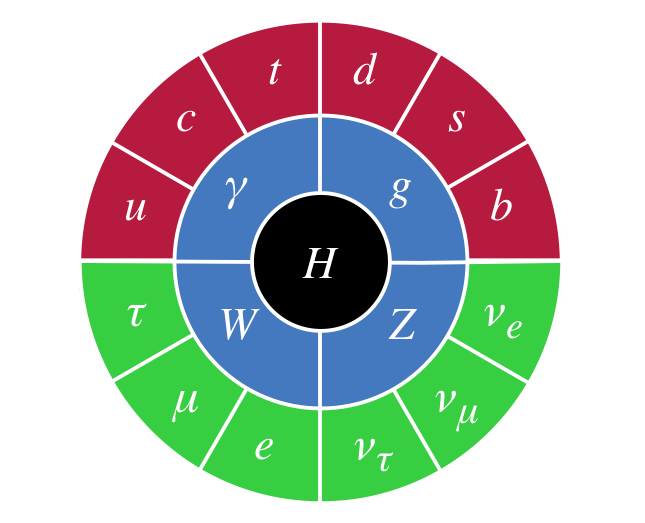
\includegraphics[width=.45\textwidth]{pics/sm_model_particles}
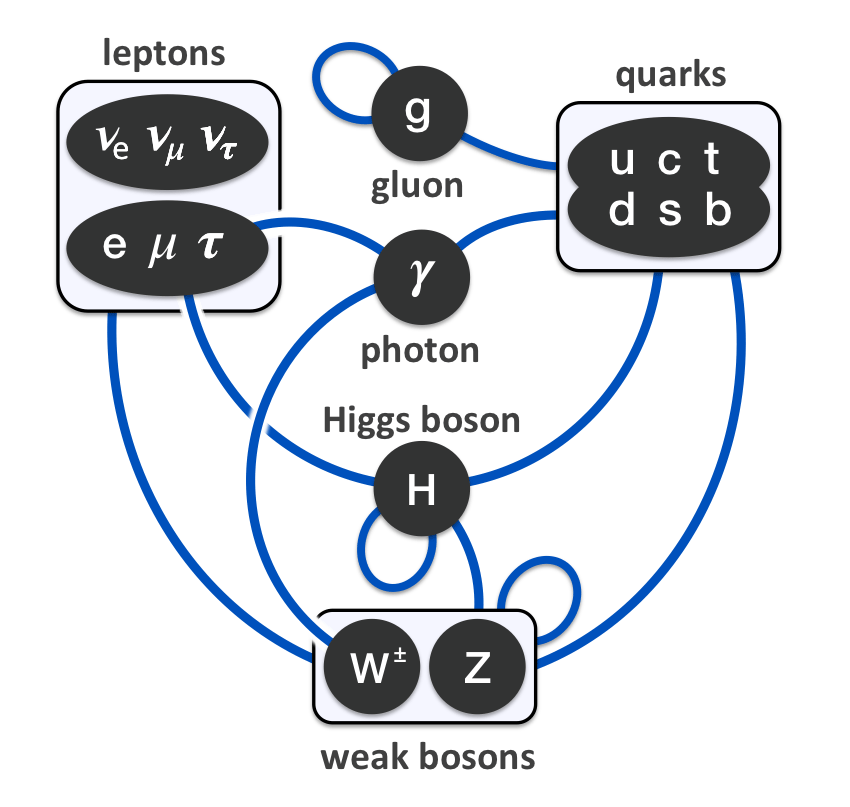
\includegraphics[width=.45\textwidth]{pics/principal_interactions}
\caption{ (Left) A representation of the particle content of the standard model. 
The inner circle is the unique scalar higgs field. The next ring consists of the 
gauge bosons. The outer ring are the fermonic fields broken into quarks and leptons. (Right) Lines drawn between particles show the fundamental interaction terms in the theory. Higher order effects can generate interactions not shown here (such as $h\rightarrow \gamma\gamma$ which is generated through a top quark loop.}
\end{center}
\end{figure}

\subsubsection{Gauge Sector}

The gauge sector consists of the field stress energy tensor of the 3 corresponding types of gauge bosons:
 $G^i$ (gluons of the color force), $W^i$ ($W$'s of the weak force) and $B$ (of the weak hypercharge). Here the index $i$ enumerates their multiplicity. There are 8 gluons, 3 $W$'s and a single B. Ultimately, we will arrive have 8 gluons, $W^{\pm}$, $Z^0$, and the photon $A$ after the $SU(2)\times U(1)$ symmetry is spontaneously broken 
and the scalar field $\phi$ takes on a new vaccum state. More on this later.
\begin{equation}
\mathcal{L}_{Gauge} = - \frac{1}{4} F_{\mu\nu}^{i} F^{\mu\nu i} =  - \frac{1}{4} G_{\mu\nu}^{i} G^{\mu\nu i} - \frac{1}{4} W^{i}_{\mu\nu} W^{\mu\nu i} - \frac{1}{4} B_{\mu\nu}B^{\mu\nu} 
\end{equation}
where the double scripts correspond to the commutation relations for the gauge group algebra. 
\begin{equation}
X_{\mu\nu}^i   = [D_u X_\nu, D_\nu X_\mu] = D_\mu X_\nu^i - D_\nu X_\mu^i - g f_{ijk} X_\mu^j X_\nu^k
\end{equation}
where $g$ is the coupling constant, the $D_\mu$ terms correspond to the covariant derivative and the $f_{ijk}$ are the corresponding structure constants for the non-abelian groups that arise from the non commuting generators of the algebra. In full, the field stress tensor terms are:
\begin{align*}
G_{\mu\nu}^i &=  D_\mu G_\nu^i - D_\nu G_\mu^i - g_s f_{ijk} G_\mu^j G_\nu^k\\ 
W_{\mu\nu}^i &=  D_\mu W_\nu^i - D_\nu W_\mu^i - g \epsilon_{ijk} W_\mu^j W_\nu^k\\ 
B_{\mu\nu} &=  D_\mu B_\nu - D_\nu B_\mu
\end{align*}
Here the  $f_{ijk}$ terms are the structure constants for the SU(3) transformations 

After electroweak symmetry breaking, when these terms are written in terms of the mass eigenstates of the theory, we generate the self-interactions of the gauge bosons such as the triple and quartic gauge couplings as 
shown in (Table. \ref{tab:interactions}). 

\subsubsection{Fermion Sector}

The fermion sector consists of the kinetic energy terms for each quark (up and down types) and leptons (lepton, neutrinos) in the standard model.
The left handed quarks transform as an SU(2) doublet:
\begin{equation}
q_{mL\alpha} = \left( \begin{array}{c} u_{m\alpha}  \\ d_{m\alpha} \end{array} \right)_L \text{ and } l_{mL} = \left( \begin{array}{c} \nu_{m}  \\ e^{-}_{m} \end{array} \right)_L 
\end{equation}
where the subscript $m$ denotes the family (1st, 2nd and 3rd generation) and $\alpha$ denotes the color charge (red, green, and blue).
As the $SU(2)_L$ symmetry only acts on the left handed fermions we further separate the fermion sector into left and right components:
\begin{align*}
\mathcal{L}_{fermion,L} &= \bar{q}_{mL} i \gamma^\mu D_\mu q_{mL} + \bar{l}_{mL} i \gamma^\mu D_\mu l_{mL}\\
\mathcal{L}_{fermion,R} &=  \bar{u}_{mR} i \gamma^\mu D_\mu u_{mR} 
+ \bar{d}_{mR} i \gamma^\mu D_\mu d_{mR} + \bar{e}_{mR} i \gamma^\mu D_\mu e_{mR} + \bar{\nu}_{mR} i \gamma^\mu D_\mu \nu_{mR}
\end{align*}

\subsubsection{Yukawa Sector}

The yukawa sector consists of terms coupling 
\begin{align*}
\mathcal{L}_{Yukawa} = - \sum_{m,n=1}^3 \left [ y^u_{mn} \bar{q}_{mL} \tilde{\phi} u_{nR} + y^d_{mn} \bar{q}_{mL} \phi d_{nR}  + y_{mn}^e \bar{l}_{mL} \phi  e_{nR}  \right ] + (h.c) 
\end{align*}
The sum is taken over families $n,m$. The single scalar field $\phi$ in two ways: $\phi = ( \phi^+ , \phi^0)$ and $\phi$ after
a SU(2) gauge transformation $\tilde{\phi} = i \tau^2 \phi^\dagger = \epsilon \phi^\dagger = 
(\phi^\dagger , -\phi^-)$. These terms need to be included such that we will
 later be able to generate mass terms for the up type quarks during electroweak symemtry breaking. The reason
we would not able to write these terms is they would violate weak hypercharge gauge invariance.  Similarlly, 
we can not write explicit mass terms $m\bar{u}_L u_R + (h.c.)$ since the left and right particles have
different hyperchage. To generate a mass term with the field $\phi$, we would have hypercharges
\begin{align*}
\bar{q}_{mL} \phi u_{nR} \implies Y= -\frac{1}{6} + \frac{1}{2} + \frac{2}{3} = 1 \neq 0
\end{align*}
Whereas using $\tilde{\phi}$ which transform as the adjoint representation
\begin{align*}
\bar{q}_{mL} \tilde{\phi} u_{nR} \implies Y= -\frac{1}{6} - \frac{1}{2} + \frac{2}{3} = 0
\end{align*}

The yukawa sector  contains a large number of the free parameters in the standard model (13 of 19). 
The individual masses of each fermion and lepton are generated by the $y_{ij}$
terms which are set to agree with experimental values (9 free parameters). These parameters 
also set the coupling of the corresponding interaction strength with the higgs boson after electroweak symmetry
breaking.

The yukawa couplings also also implicitly includes parameters characterizing the mis-match 
mixing betwen the quark flavor and mass eigeinstates which occur after electroweak 
symmetry breaking (4 parameters). Had the mass flavor states been aligned, we would not the two family indices to 
be able to generate mass terms after EWSB. The mixing is characterized by  the 3x3 unitary
 Cabibbo-Kobayashi-Maskawa (CKM) matrix $V^{CKM}$. The convention is chosen that flavor
 states $u^I$ for up type quarks are aligned with the mass states $u$ and the down type quarks are
rotated through the transformation $d^I_i = V^{CKM}_{ij} d_{j}$. From the unitarity condition, the matrix can be parameterized in 4 parameters: three mixing angles $\theta_{12}, \theta_{23}, \theta_{13}$ and a CP violating phase $\delta$:

\begin{align*}
\begin{pmatrix}  d^I \\ s^I \\ b^I \end{pmatrix} &=
 \begin{pmatrix} V_{ud} & V_{us} & V_{ub} \\ V_{cd} & V_{cs} & V_{cb} \\ V_{td} & V_{ts} & V_{tb} \end{pmatrix} 
\begin{pmatrix}  d \\ s \\ b \end{pmatrix}  \\
&= \begin{pmatrix} c_{12}c_{13} & s_{12} c_{13} & s_{13} e^{-i\delta} \\ 
-s_{12}c_{23} - c_{12}s_{23}s_{13}e^{i\delta} & c_{12} c_{23} - s_{12} s_{23} s_{13} e^{i\delta} & s_{23} c_{13} \\
s_{12}s_{23} - c_{12} c_{23} s_{13} e^{i\delta} & -c_{12}s_{23}-s_{12}c_{23}s_{13}e^{-\delta} & c_{23}c_{13}  \end{pmatrix} 
\begin{pmatrix}  d \\ s \\ b \end{pmatrix} 
\end{align*}
where $c_{ij} = \cos \theta_{ij}$ and $s_{ij} = \sin \theta_{ij}$. It is important to note a similar matrix exists for leptons
and is used for the study of neutrino oscillations known as the Pontecorvo-Maki-Nakagawa-Sakata (PMNS) matrix but is assumed to
be $1$ in the standard model. 

\subsubsection{Higgs Sector and Electroweak Symmetry Breaking} 

The higgs sector consists of terms related to the single scalar field $\phi$ 
that transforms as a doublet of $SU(2)$ as $\phi = (\phi^+, \phi^0)$
 and $\phi^\dagger = (\phi^- , (\phi^0)^\dagger)$ noting that
 $\phi^\dagger \phi = \phi^+\phi^- + (\phi^0)^\dagger \phi^0$
\begin{equation}
\mathcal{L}_{higgs} = (D^\mu \phi)^\dagger(D_\mu \phi) + \mu^2 \phi^\dagger \phi + \lambda (\phi^\dagger \phi)^2 
\end{equation}

This sector contains only two free parameters: $\mu$ and $\lambda$. The two parameters set the minimum and stability of the vaccum of the theory and set the masses of the fermions and gauge bosons after electroweak symmetry breaking. 

\begin{figure}
\begin{center}
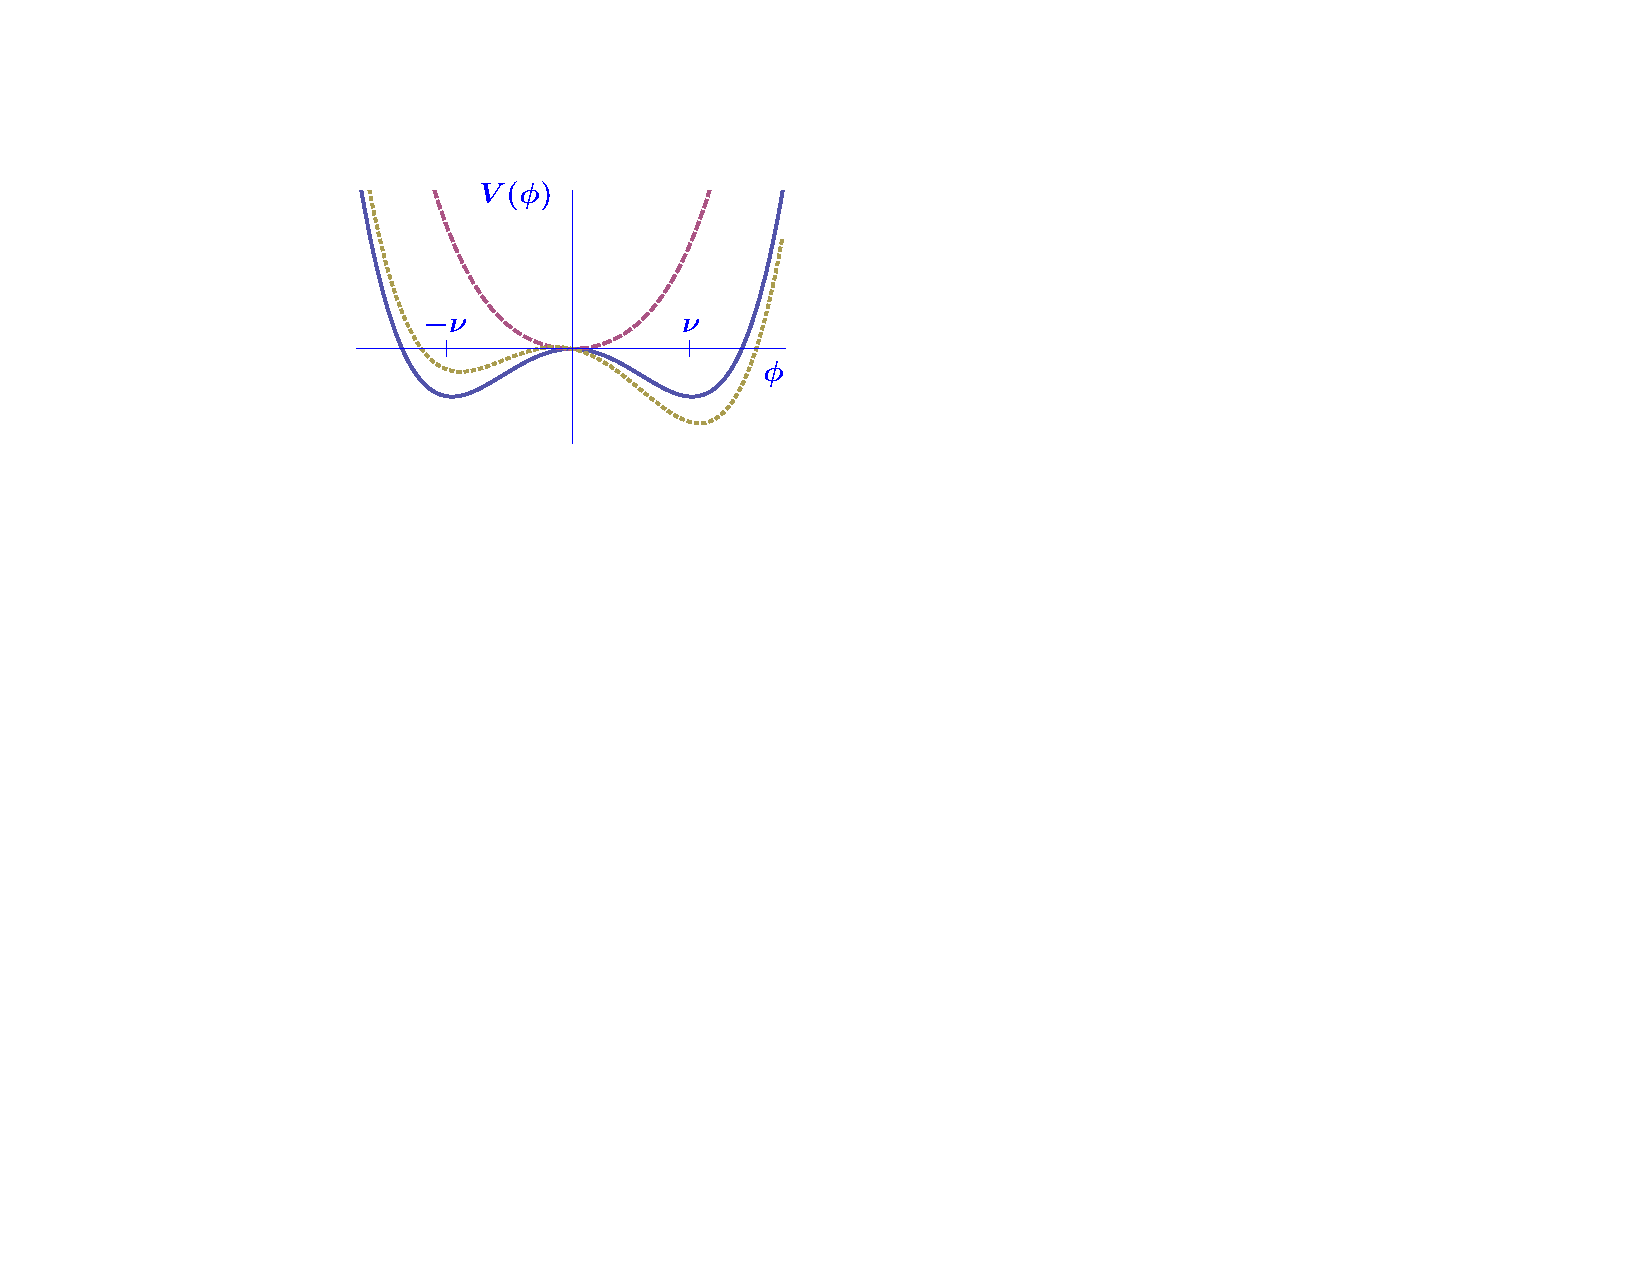
\includegraphics[width=.45\textwidth]{pics/scalar_potential}
\end{center}
\caption{Shape of the $\phi$ potential varying the values of $\mu^2$}
\label{fig:scalar_potential}
\end{figure}

The shape of the vaccum potential is determined by this sector and essential to the nature of electroweak symmetry
breaking and the stability of the vaccum. We require that $\lambda>0$ such that the potential is bounded from below, however $\mu^2$ can be arbitrary. If $\mu^2 >0$ we would have a minimum at $\phi=0$ and $\langle \phi \rangle =0$. If $\mu^2 < 0$ the theory becomes unstable with 

As the field $\phi$ is a complex scalar field we can parameterize the field in terms
 of real scalar fields $\phi_1$ and $\phi_2$:
\begin{align*}
\phi = \frac{1}{\sqrt{2}} ( \phi_1 + i \phi_2) \text{ and } \phi^\dagger = \frac{1}{\sqrt{2}} ( \phi_1 - i \phi_2)
\end{align*}
Given this parameterization, the potential becomes:
\begin{align*}
V(\phi) = \frac{1}{2}\mu^2 ( \phi_1^2 + \phi_2^2 ) + \frac{\lambda}{4} ( \phi_1^2 + \phi_2^2)^2 
\end{align*}
letting $x = \phi_1^2 + \phi_2^2$ and minimizing $\frac{\partial V}{\partial x } = 0$ we find $x_{min} = \nu$. As
the vaccum is stable the theory will move to this minimum (Figure \ref{fig:scalar_potential}). Expanding
around the new vaccum $\phi_1' = \nu + \phi_1$ and $\phi_2' = \phi_2$ we obtain the new vaccum potential terms
relative to the unbroken theory:
\begin{align*}
V(\phi') = \frac{-\mu^2}{4\lambda} - \mu^2 (\phi_1^2) + \lambda \nu \phi_1 (\phi_1^2 +\phi_2^2) + \frac{\lambda}{4}(\phi_1^2 + \phi_2^2)^2 
\end{align*}
The first of these terms is a cosmological constant and does not affect the dynamics of the theory. However,
such a constant would be relevant gravitational theories where gravity couples to energy.
The second term is the mass term for the higgs field. The third and fourth corresponds to the cubic
 and quadratic self interactions. 

\begin{figure}
\begin{center}
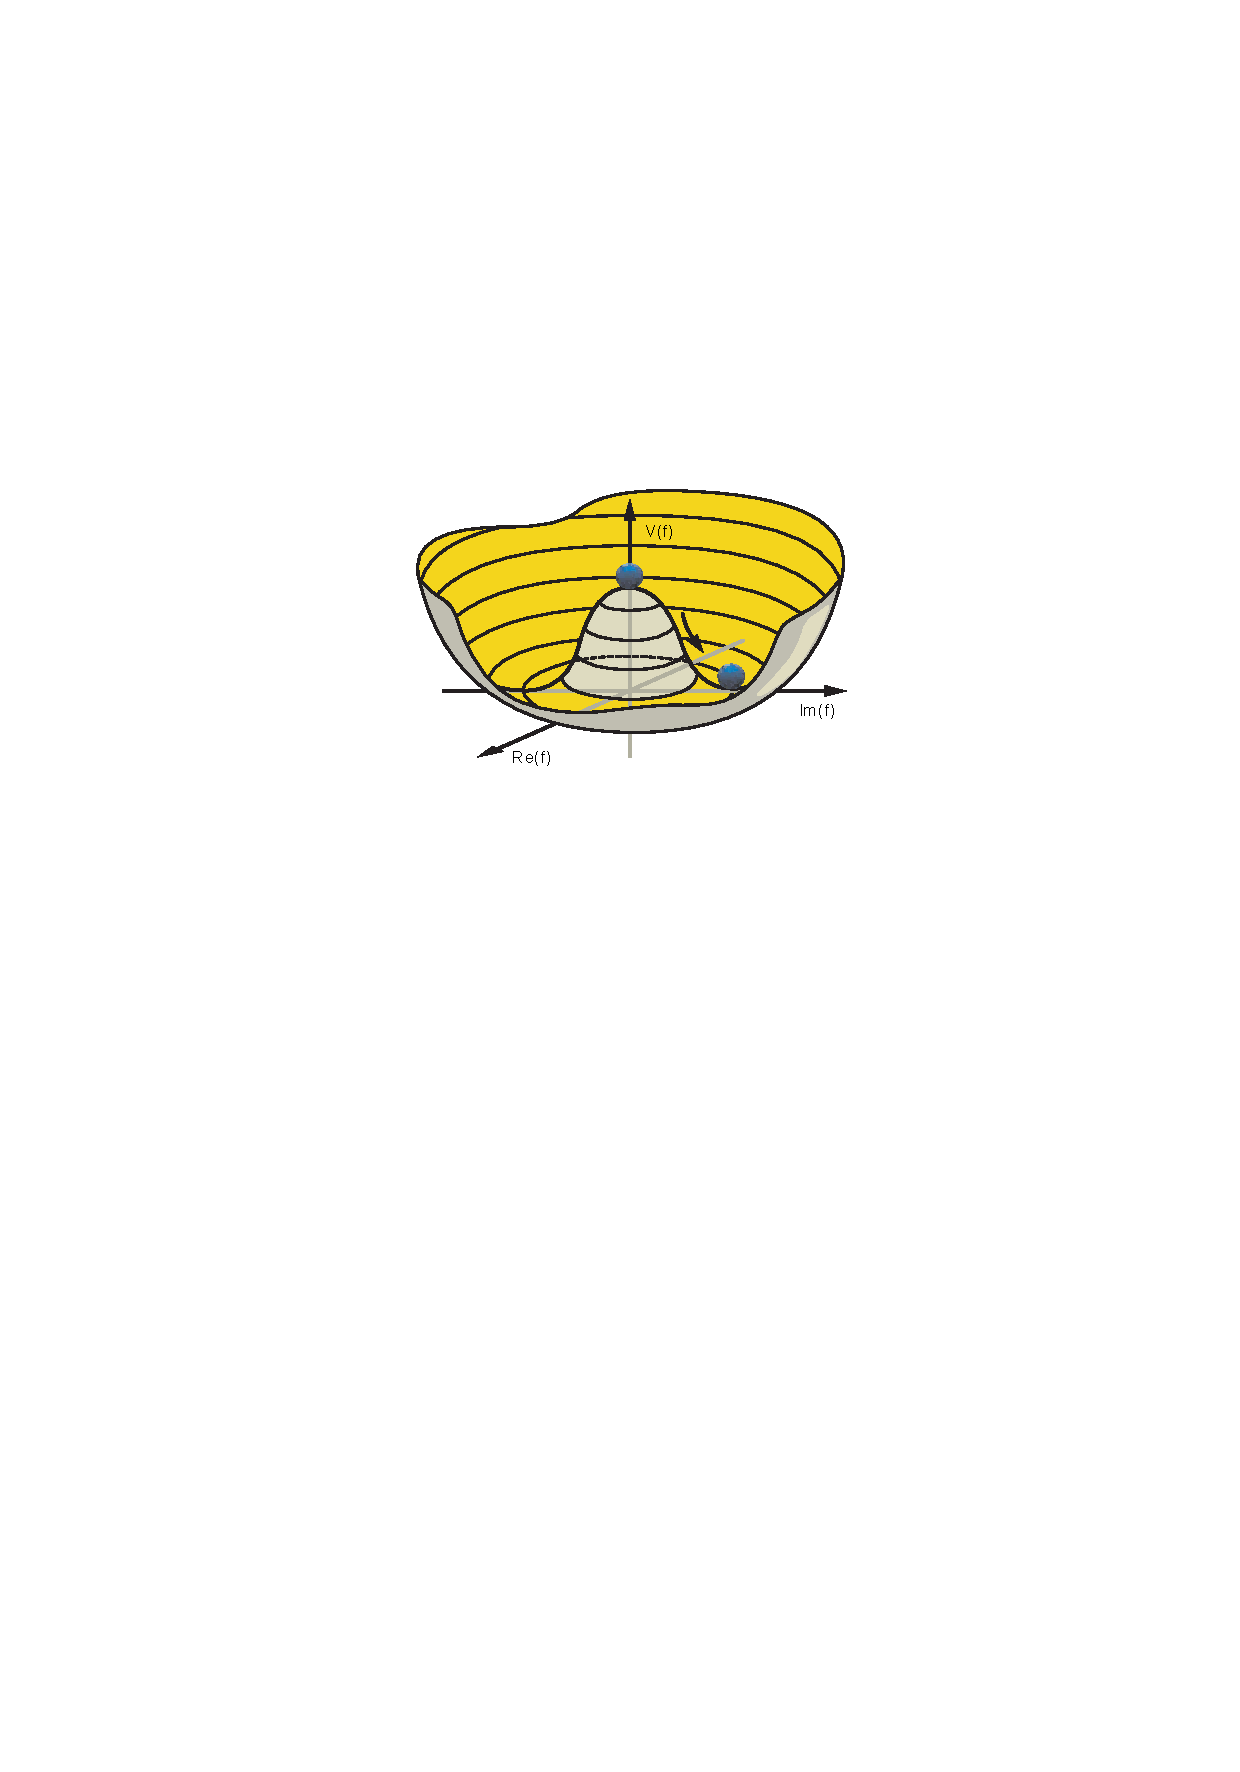
\includegraphics[width=.55\textwidth]{pics/higgs_potential}
\end{center}
\caption{The higgs potential exhibiting spontaneously broken symmetry, where the expected vaccum expectation
value has moved from the $0$ of the theory to $\nu$ in the broken theory}
\end{figure}

If we consider the kinetic term for the field $\phi$ at the now borken vaccum $\langle \phi \rangle = (0 , \nu)$ in the gauged theory we find:
\begin{align*}
(D^\mu \phi)^\dagger (D_\mu \phi) = \frac{1}{\sqrt{2}} \left (\begin{array}{cc} 0  & \nu \end{array} \right )  \left | \partial_\mu + i g \frac{\tau}{2} \cdot W_\mu + i \frac{g'}{2} B_\mu \right|^2  \frac{1}{\sqrt{2}} \left (\begin{array}{c} 0 \\ \nu \end{array} \right ) 
\end{align*}
Considering the weak gauge term:
\begin{align*}
\tau \cdot W  = \left (\begin{array}{cc} W_{\mu,3} & W_{\mu,1} - i W_{\mu,2}  \\ W_{\mu,1}+ i W_{\mu,2} & - W_{\mu,3} \end{array} \right )
\end{align*}
adding in the diagonal $B_\mu$ terms and taking the square (ignoring the partial terms) 
\begin{align*}
(D^\mu \phi)^\dagger (D_\mu \phi) \supset \frac{\nu^2}{8} \left [g^2 (W_1^2 + W_2^2) + (g' B_\mu - g W_{\mu,3})^2 \right]
\end{align*}
Now if we perform a redefinition of the gauge fields into mass eigenstates we arrive at a clean expression:
\begin{align*}
W_{\mu}^{\pm} &= \frac{1}{\sqrt{2}}( W_{\mu,1}  \pm i W_{\mu,2} )  \\
A_{\mu} &= \frac{1}{\sqrt{g^2 + (g')^2}} (g' W_{\mu,3} + g B_\mu) = \sin \theta_W W^3_\mu + \cos \theta_W B_\mu \\
Z_{\mu} &= \frac{1}{\sqrt{g^2 + (g')^2}}( g' B_\mu - g W_{\mu,3}) = \sin \theta_W B_\mu - \cos \theta_W W_\mu^3 
\end{align*}
Here we have defined the electroweak mixing angle $\theta_W$ in terms of a right triangle with legs $g$ and $g'$. With this substitution,
\begin{align*}
(D^\mu \phi)^\dagger (D_\mu \phi) &\supset \frac{\nu^2 g^2}{4} W_{\mu}^{-} W_{\mu}^{+} + \frac{(g+g')\nu^2}{8} Z_\mu^2  + (0 \times A_\mu^2) \\ 
&= \frac{1}{2} m_{W}^2 W_\mu^- W_\mu^+ + \frac{1}{2} m_Z^2 Z_\mu^2  + (0 \times A_\mu^2)
\end{align*}
Electroweak symmetry breaking has generated the mass terms for the gauge bosons! 
$m_{W^{\pm}} = \frac{\nu g}{\sqrt{2}} = 80.385$~[GeV],
$m_Z = \frac{\nu}{2}\sqrt{g+g'} = \frac{m_W}{\cos \theta_W} = 91.1876$~[GeV]  and the massless photon $A_\mu$. 


\subsection{Maxwell's Laws} 

After electroweak symmetry breaking we would like to perform a sanity check that we can deduce the well studied
 equations governing electrodynamics from the QFT description. Keeping only the terms that contain the field $A_\mu$:
\begin{align*}
\mathcal{L}_{EM} = -\frac{1}{4} F_{\mu\nu} F^{\mu\nu}  - ie \bar{\psi} \gamma^\mu A_\mu \psi \text{ for } F_{\mu\nu} = \partial_\mu A_\nu - \partial_\nu A_\mu 
\end{align*}
where by definition $F_{\mu\nu} = \partial_\mu A_\nu - \partial_\nu A_\mu$. Applying the left side of Euler-Lagrange we find:
\begin{align*}
\partial_\mu \left (\frac{\partial \mathcal L}{\partial(\partial_\mu A_\nu)} \right) &=  
-\frac{1}{2}\partial_\mu \left [ \left (\frac{\partial}{\partial(\partial_\mu A_\nu)} F_{\mu\nu} \right) F^{\mu\nu} \right ] 
= -  \partial_\mu F^{\mu\nu}
\end{align*}
The other term is simply $\frac{\partial \mathcal L}{\partial A_\mu} = -ie \bar \psi \gamma^\mu  \psi = - J^\mu = -(\rho, \vec J)$. Where $\rho$ is charge
density and $\vec J$ is current. This yields our first equation:
\begin{equation}
\partial_\nu F^{\nu\mu} = J^\mu
\end{equation}
recognizing the field tress tensor is antisymmetric we can apply a partial derivative and contract with the indicies of the 4 dimensions anti-symmetric symbol
to obtain:
\begin{equation}
\epsilon_{\theta\rho\mu\nu} \partial_{\rho} F_{\mu\nu} = 0 
\end{equation}
Using these two laws we first see that the electric and magnetic field, $E$ and $B$, can be
defined in terms of the field stress tensor
\begin{align*}
F_{0i} = \partial_0 A_i - \partial_i A_0 = -\frac{\partial A}{\partial t} - \nabla \Phi = E
\end{align*}
and for the magnetic field we consider 
\begin{align*}
\epsilon_{ijk}B^k &= \epsilon_{ijk} \epsilon_{klm} \partial_l A_m = \epsilon_{kij} \epsilon_{klm} \partial_l A_m = (\delta_{il} \delta_{jm} - \delta_{im}\delta_{jl}) \partial_l A_m = \partial_i A_j - \partial_j A_i = F_{ij}
\end{align*}
From the first current law we immediately obtain two of maxwells laws:
\begin{align*}
\partial_i F^{0i} = \rho \implies \nabla \cdot E = \rho
\end{align*}
and for the second we separate the sum between space and timelike components:
\begin{align*}
\partial_i F^{ji} + \partial_0 F^{j0} = J^j\\
\epsilon_{jik} \partial_i B_k - \partial_0 E^j = J^j\\
\nabla \times B - \frac{\partial E}{\partial t} = \vec J
\end{align*}
The remaining two laws come from manipulations of the antisymmetry of the field stress tensor:
\begin{align*}
0 = \epsilon_{0ijk} \partial_i F^{jk} =
\epsilon_{0ijk} \partial_i \epsilon_{0jkl} B_l =
\epsilon_{jk0i}  \epsilon_{jkl0} \partial_i B_l  =
-\delta_{il} \partial_i B_l  \\
\implies \nabla \cdot B = 0
\end{align*}
If we examine the time component of the field stress tensor we find the last equation in terms of $E$ and $B$
\begin{align*}
\epsilon_{\mu\nu0\sigma} \partial_\nu F^{0\sigma} + \epsilon_{\mu\nu i\sigma} \partial_\nu F^{i\sigma}&= 0 \text { for } i=1,2,3\\
\epsilon_{0\sigma\mu\nu} \partial_\nu E^{\sigma} + \epsilon_{\mu\nu i\sigma}  \epsilon_{0i\sigma k} \partial_\nu B_k&= 0 \text{ where } k\neq 0\\
\end{align*}
The first term gives us $\nabla \times \vec E$ lets separatly expand the second term by permuting the $\epsilon$ indicies
\begin{align*}
\epsilon_{i\sigma \mu\nu}  \epsilon_{i\sigma k 0}  \partial_\nu B_k&= 0 \text{ where } k\neq 0\\
(\delta_{uk} \delta_{\nu 0} - \delta_{\mu 0} \delta_{\nu k} )  \partial_\nu B_k&= 0\\
 \partial_0 B_\nu - \partial_k B_k&= 0\\
\frac{\partial \vec B}{\partial t} - \nabla \cdot \vec B&= 0\\
\frac{\partial \vec B}{\partial t}&= 0\\
\end{align*}
In the last line we have used the previous law that $\nabla \cdot \vec B = 0$. Combining the two terms we obtain the 
final law
\begin{align*}
\nabla \times \vec E + \frac{\partial \vec B}{\partial t}&= 0\\
\end{align*}
Don't forget that the assumptions to get here were simply the existence of energy terms for the field stress tensor 
and the fermonic field $\psi$ (here the electron) and geometric arguments about the continutity in the derivative 
under the local $U(1)$ gauge symmetry in the Lagrangian. Everything we historically understood
about about electromagnetism naturally arises. This even (obviously) includes the curiousity of electromagnetism that
the equations remain unchanged under a gauge transformation vector field $\vec A$. However, in a gauge theory 
this is the fundamental princple rather than a consequence of the form of Maxwell's equations. 
That's just awesome. 

\subsection{Feynman Diagrams}

\begin{figure}
\begin{center}
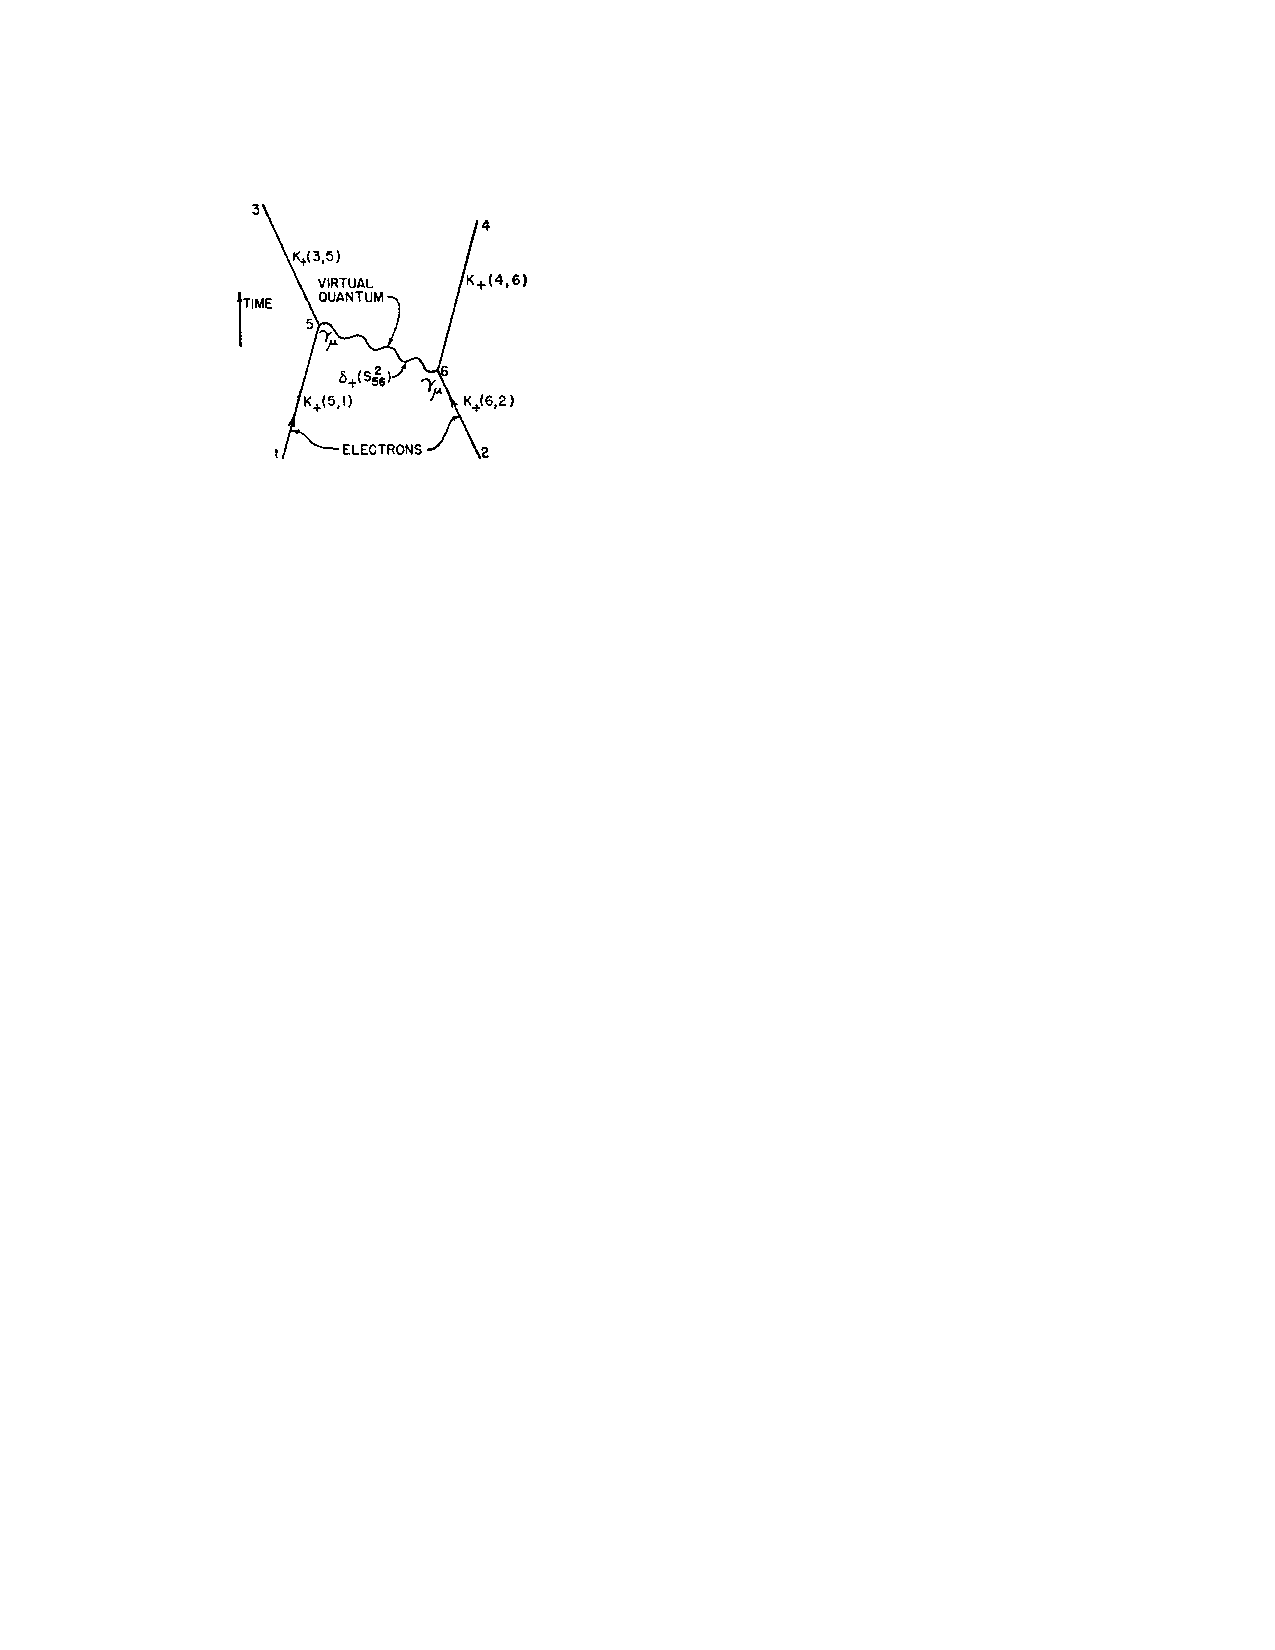
\includegraphics[width=.450\textwidth]{pics/first_diagram}
\end{center}
\caption{The feynman diagram for describing t-channel scattering of two electrons through
the exchange of a photon. This particular figure was the example used in feynman's original paper describing the pictoral representation
of calculating matrix elements. (cite-first-feynman diagram)}
\label{fig:first_diagram}
\end{figure}

Historically, the outcome of a scattering event in a quantum field theory was
 incredibly tedious to calculate. One of Feynman's greatest contributions to the field o
f particle physics was an organizational to tool group and quickly calculating terms 
in the perturbative expansion of the action. The diagrams, Feynman diagrams (Figure \ref{fig:first_diagram}), 
take the form of a directed graph of lines and vertices providing a  representation
the components needed for the ultimate calculation that was intuitive to work with. 

To calculate a given scattering amplitude, one simply constructed all of the applicable diagrams between
the incoming particles (ex. proton-proton) and the outgoing final state  (ex. $q\bar{q}$). Lines represented particles with a given momentum and vertices represented
interaction terms in the lagrangian where four-momentum convservation was enforced. Internal 
lines of the diagram, that is, neither initial nor final state particles, were virtual 
particles were space-like. 

Lets consider a simple theory with a single scalar field $\phi$ and a $\phi^3$ interaction term:
\begin{align*}
\mathcal{L} = \mathcal{L}_0 + \mathcal{L}_{int} = \frac{1}{2}(\partial_\mu \phi) (\partial^\mu \phi) + m^2 \phi^2 - \frac{\kappa}{3!} \phi^3 
\end{align*}
In the schrodinger picture of quantum mechanics the states $|\psi \rangle$  evolve in time 
according to the hamiltonian $H_S=H_0+H_{int}.$  Here $H_0$ is the free particle component and $H_{int} = - \mathcal{L}_{int}$ is the interacting component. The quantum state obeys the schrodinger equation:
\begin{align*}
i\frac{d}{dt} |\psi \rangle = H_S | \psi \rangle
\end{align*}
This gives we obtain the solution $|\psi(t,x) \rangle =  U(t,0)| \psi(0,x) \rangle$ where we define
the time evolution operator $U(t,t_0) = \exp{(-iH_S (t-t_0))}$.  The observables are constant in time
and the expected value of some operator (in our case the quantum field $\phi$) on a state
at time $t$ can be written:
\begin{align*}
\langle \phi(t,x) \rangle = \langle x,t_0 | e^{iH_S(t-t_0)} \phi(x) e^{-iH_S(t-t_0)} | x,t_0 \rangle 
\end{align*}
In the heisenburg picture, we instead absorb the time dependence into the operator, leaving the states constant.
\begin{align*}
 \phi(t,x) =   e^{iH_St} \phi(x)  e^{-iH_St}
\end{align*}
Lets define a new interacting field $\phi_I = e^{iH_0t} \phi  e^{-iH_0t}$ which evolves
 with the free hamiltonian. Now in the heisenburg picture field can be written in terms of $\phi_I$ as:
\begin{align*}
 \phi(t,x) &=   e^{iH_St}e^{-iH_0t} \phi_I(x) e^{iH_0t} e^{-iH_St} = U^\dagger(t) \phi U(t)
\end{align*}
We have defined a unitary operator $U(t)=e^{iH_0t}e^{-iH_St}$. If we apply a time derivative to $U(t)$ we find:
\begin{align*}
i\partial_t U(t) &= -e^{iH_0t}H_0 e^{-iH_St} + e^{iH_0t} H_S e^{-iH_St}\\
&= e^{iH_0t}H_{int}e^{-iH_St}\\
&= e^{iH_0t}H_{int}e^{-iH_0t}e^{iH_0t}e^{-iH_St}\\
&= H_I U(t) = \left (\frac{\kappa}{3!}\phi_I^3 \right) U(t)
\end{align*}
We have shown the time evolution operator obeys the schrodinger equation under a hamiltonian $H_{I}$, corresponding to
 $H_{int}$ in the heisenburg picture. Solving this equation, we obtain a time evolution
operator $U(t) = T\exp (-\int dt iH_I)$. The operator $T$ denotes time ordering of the time integrals for each term
in the taylor expansion of the exponential which will not necessarily commute. Since each $H_I(t)$ will be integrated against it's own dummy time variable, the time ordering operator will place $H_I(t)$ terms farther to the left, if they occur later in time. 

We have succeeded in writing the time evolution operator in terms of the field $\phi_I$ which evolves according to the free hamiltonian for which we already have a  solution expressed in terms of creation and annihilation operators:
\begin{align*}
\phi_I(\vec x, t) = \int \frac{d^4p}{(2\pi)^3\sqrt{2E}} \left [  a_p e^{ipx} + a_p^\dagger e^{-ipx} \right ]
\end{align*}
Now when we would like to compute the matrix element of $\phi\phi$ scattering, we expand the time evolution operator:
\begin{align*}
U(t,0) &= 1 - i \int_0^t H_I(t)  - \frac{1}{2} \int_0^t dt \int_0^{t'} dt' T\{ H_I(t) H_I(t')\} \ldots \\
&= 1 - i \int d^4x \frac{g}{3!}\phi^3(x)  - \frac{1}{2} \frac{g^2}{3!3!} \int d^4x \int d^4x' T \{ \phi^3(x) \phi^3(x') \}  \ldots 
\end{align*}
When we calculate the matrix element $\mathcal{M}_{if} = \langle p_3^fp_4^f|U(-\infty,\infty)|p_1^i p_2^i \rangle$ and $\kappa<1$ the theory is perturbative and first non-zero term will dominante the ultimate calculation. 
For $2\rightarrow 2$ scattering this 
term will be at order $\kappa^2$ and is computed by expanding the fields in terms
of the creation and annihilation operators. Since $a|0\rangle = \langle 0 | a^\dagger = 0$ the only terms which will contribute will be the terms with equal numbers of creation and annihilation operators coming from the $\phi^3(x)\phi^3(x')$ term. 


Rather than arduously expanding all of these fields, we use a result known as Wick's Theorem in combination
with the LSZ reduction formula for converting
the time ordered product into a series of pair-wise contractions between the individual fields. 
A contraction is defined for a field $\phi$ decomposed into its positive and negative 
frequency components $\phi_I = \phi^+_I +\phi^-_I$ where the $+$ field contains the annihilation operator term, and $-$ the creation operator term.
%\contraction{}{}{$\phi$}{$(x)$}{$\phi$}(y)
\begin{align*}
\begC1{\phi}\conC{(x)}\endC1{\phi}(y)  = [\phi^+(x),\phi^-(y)] \text{ if } x^0 > y^0 \text{ else } [\phi^+(y),\phi^-(x)] 
\end{align*}
Given this definition, we state Wick's theorem as:
\begin{align*}
T[\phi_1(x_1) \ldots \phi_N(x_N) ] = N \left [ \phi_1(x_1) \ldots \phi_N(x_N) + \text{ all possible contractions }      \right ]
\end{align*}
Where $N$ is the normal ordering operator which operates on a sequence of creation and annihilaiton operators by moving
all creation operators to the left and annihilation operators to the right. By normally ordering a term
in the expansion that does not appear, we can eliminate all uncontracted terms. In lieu of a proof of Wick's theorem, 
we can consider the process of taking the original term and moving creation operators to the left using commutation relations:
\begin{align*}
a_1a_2a^\dagger_3a_4 = a_1 a_3^\dagger a_2 a_4 + a_1 [a_2,a_3^\dagger] a_4 
\end{align*}
each time we move a field, we pick up a commutator between two elements. 


\begin{itemize}
\item External lines: 1 for scalars 
\item Internal lines: $\Delta(p) = \frac{i}{p^2 - m^2+i\epsilon}$
\item Vertices: $-i\kappa$
\item Symmetry Factors: divide by the symmetry factor 
\item Momentum Convservation: require that four momentum is conserved at each vertex 
\item Integrate over undetermined momentum 
\end{itemize}

\begin{figure}
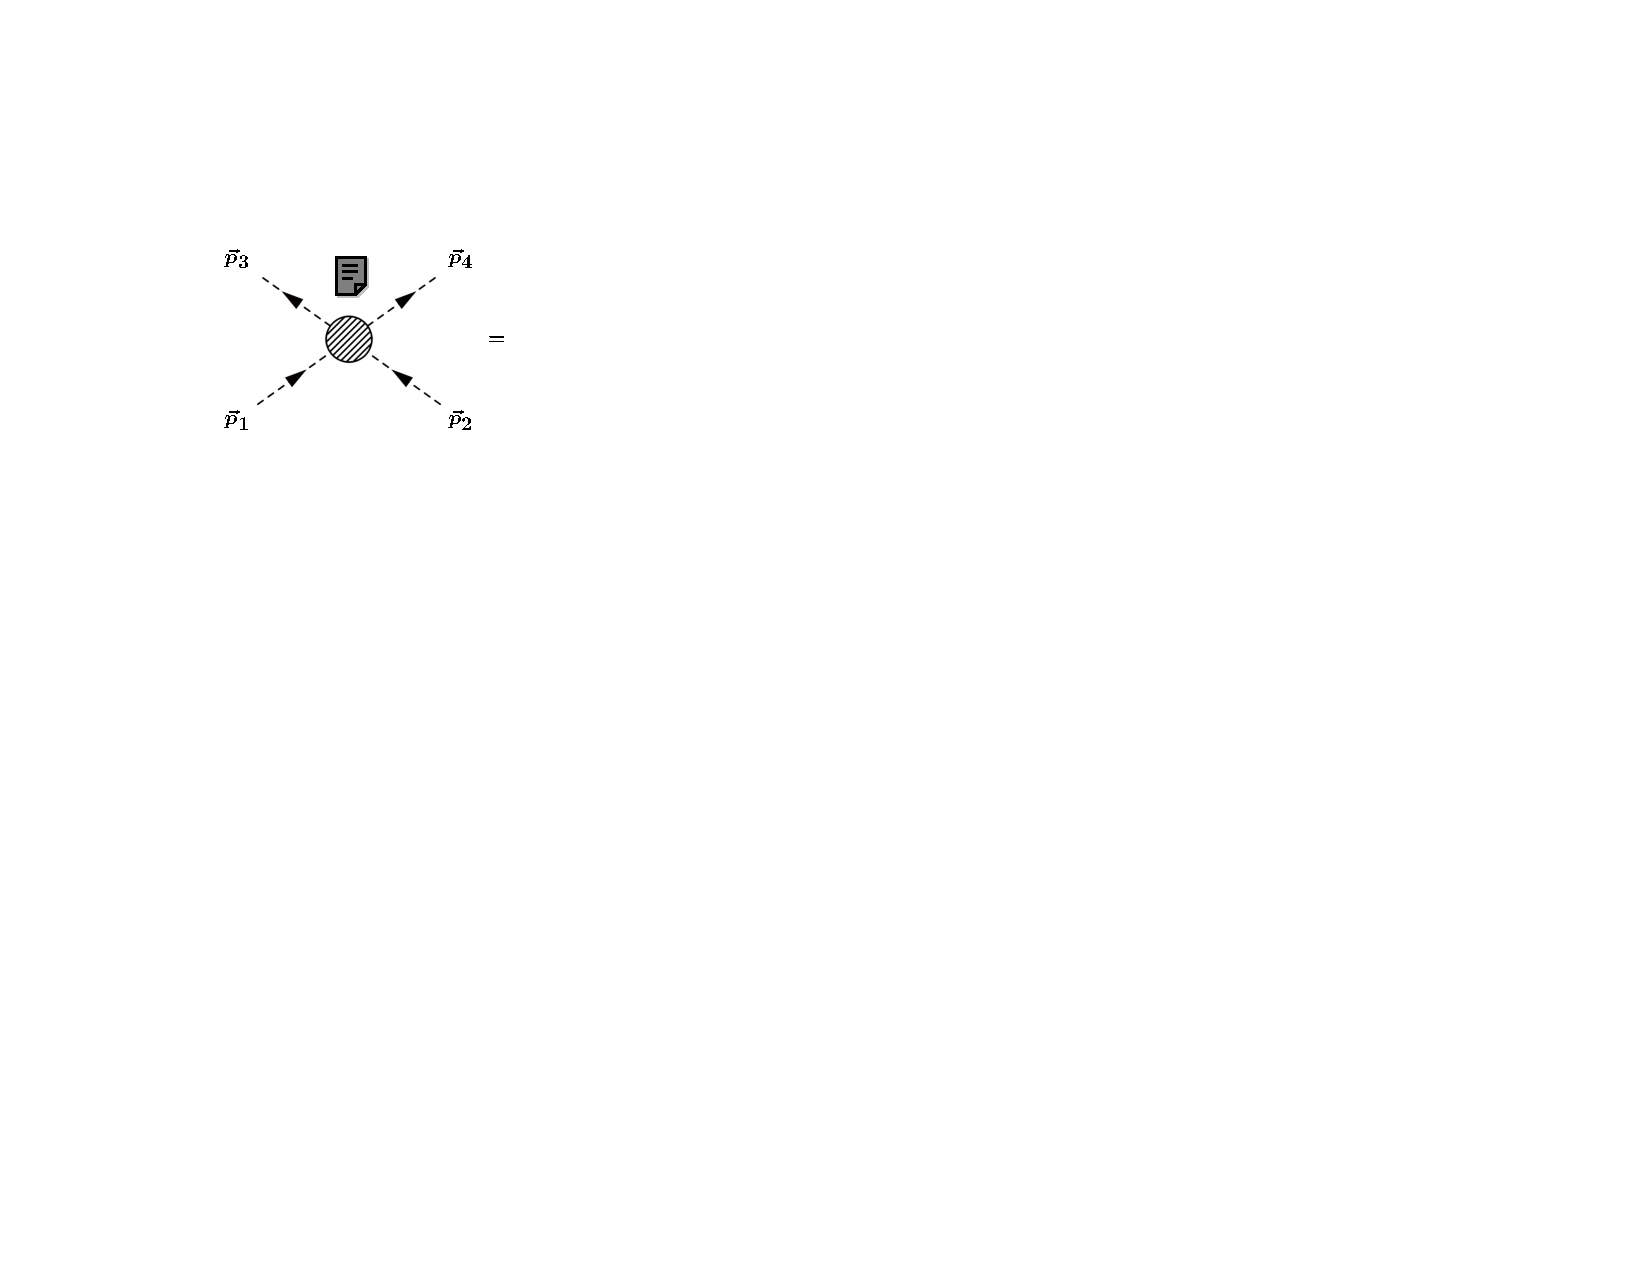
\includegraphics[width=.31\textwidth]{pics/interaction}\\
\begin{center}
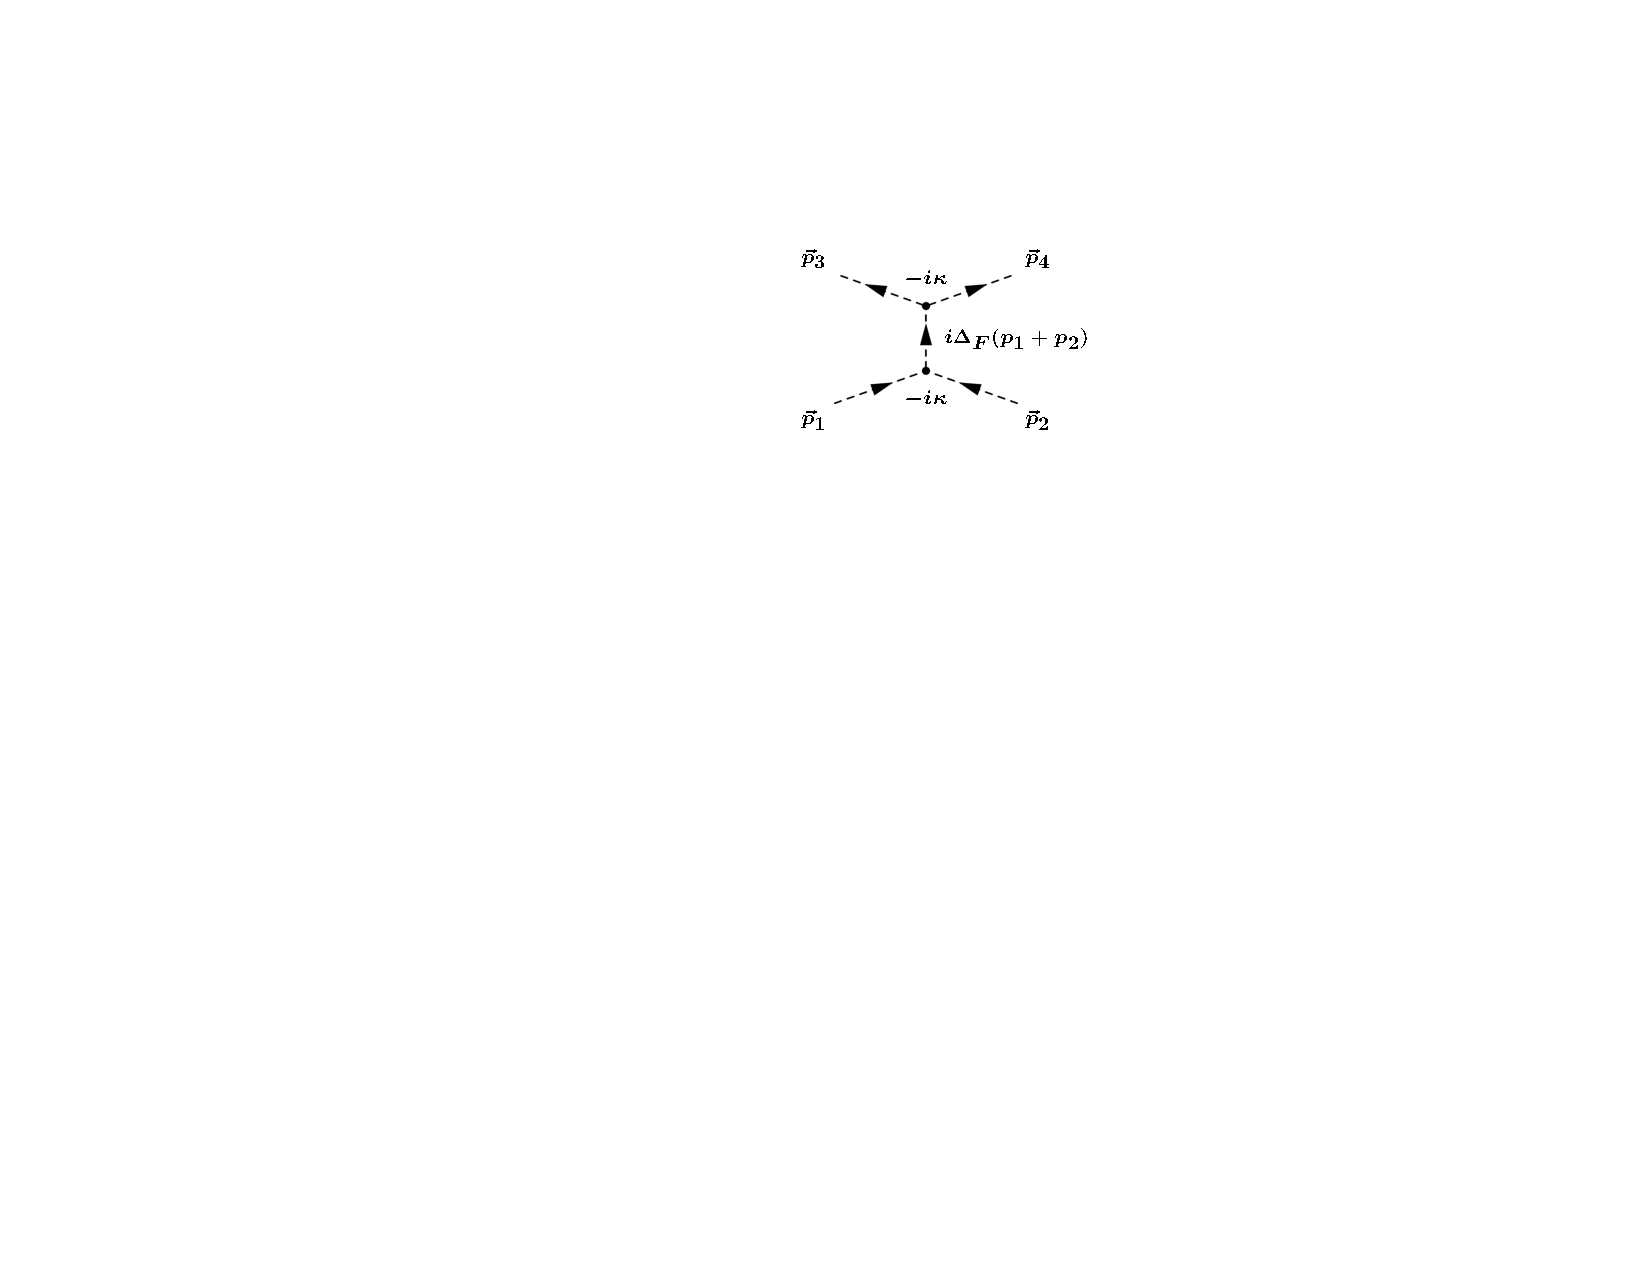
\includegraphics[width=.31\textwidth]{pics/s_diagram}
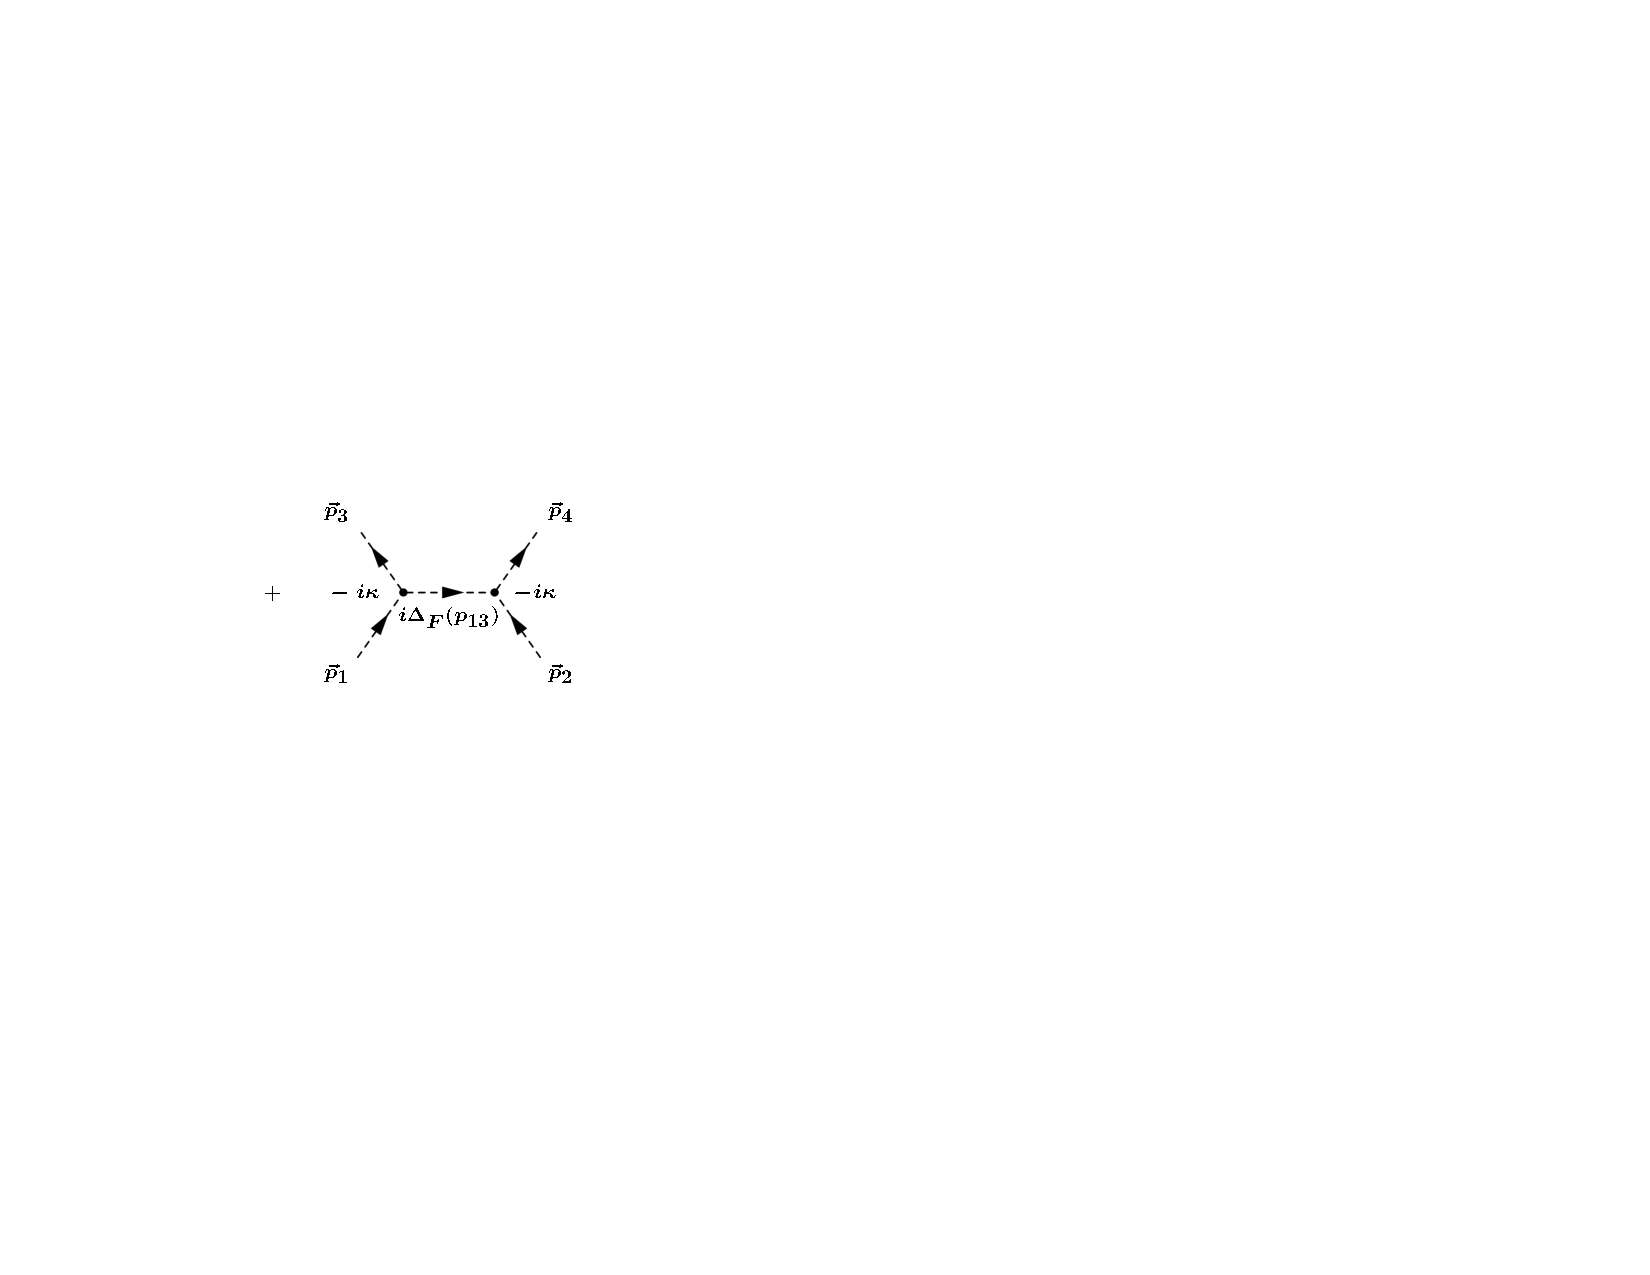
\includegraphics[width=.31\textwidth]{pics/t_diagram}
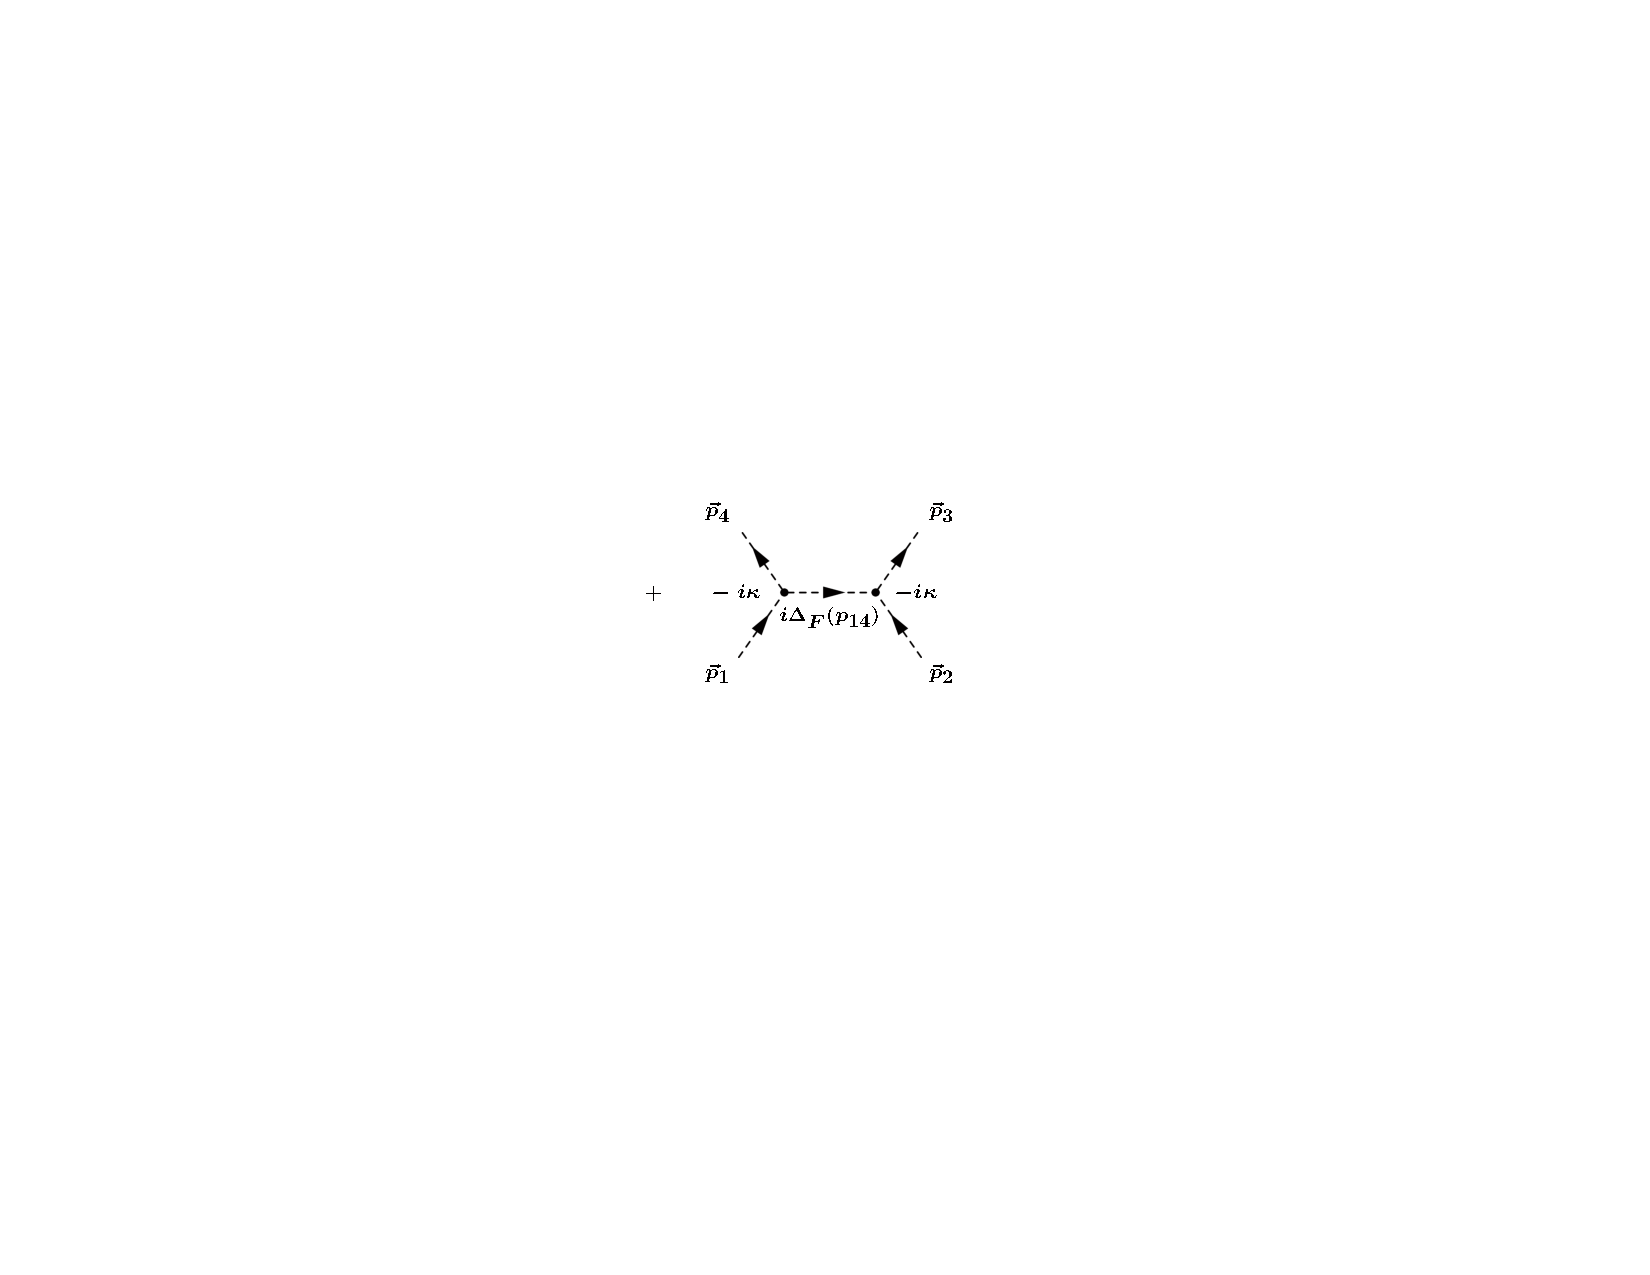
\includegraphics[width=.31\textwidth]{pics/u_diagram}
\end{center}
\caption{The 3 diagrams corresponding to $\phi\phi\rightarrow \phi\phi$ scattering at tree level (leading order). Time
is directed vertically. 
 }
\end{figure}

For simple tree level scattering (up to order $g^2$) for $\phi_1 \phi_2 \rightarrow \phi_3 \phi_4$ the 
amplitude is given by 3 diagrams where a virtual $\phi$ is exchanged. 
Introducing the Mandlestam variables:
\begin{align*}
s&=(p_1+p_2)^2  = 4(p^2+m^2) = E_{cm}^2 \\
t&=(p_1-p_3)^2  = -2p^2(1-\cos\theta)\\
u&=(p_1-p_4)^2 = -2p^2(1+\cos\theta) 
\end{align*}
Here the scattering angle $\theta$ has been introduced defined as $\vec p_i \cdot \vec p_f$ in the center 
of mass frame. Summing the  diagrams appropriately labeled $s,t,$ 
and $u$-channel we calculate the unsquared amplitude. 
\begin{align*}
\mathcal{M} = (-i\kappa)^2\left( \frac{i}{s-m^2} + \frac{i}{t-m^2} + \frac{i}{u-m^2} \right)
\end{align*}
The rate of this process is proportional to the When the value of $g$ is perturbative this is the leading contribution to the 

\subsection{Radiative Corrections and Renormalization} 

\begin{figure}
\begin{center}
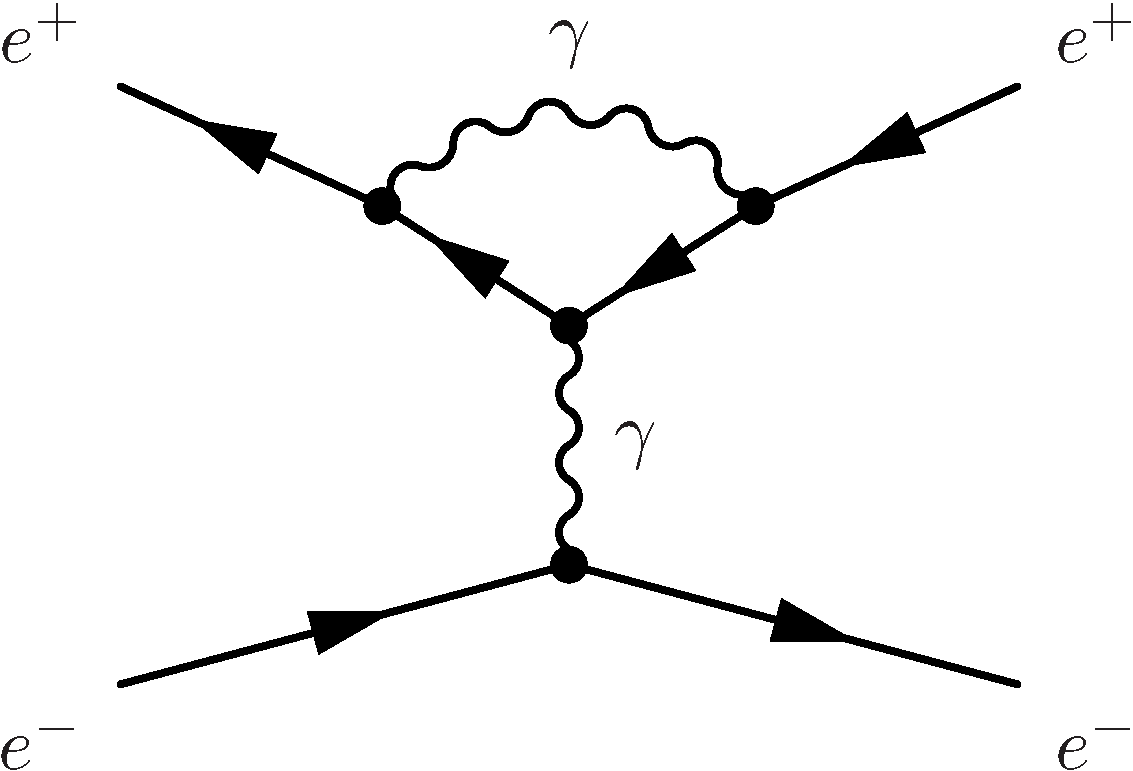
\includegraphics[width=.3\textwidth]{pics/vertex_correction}
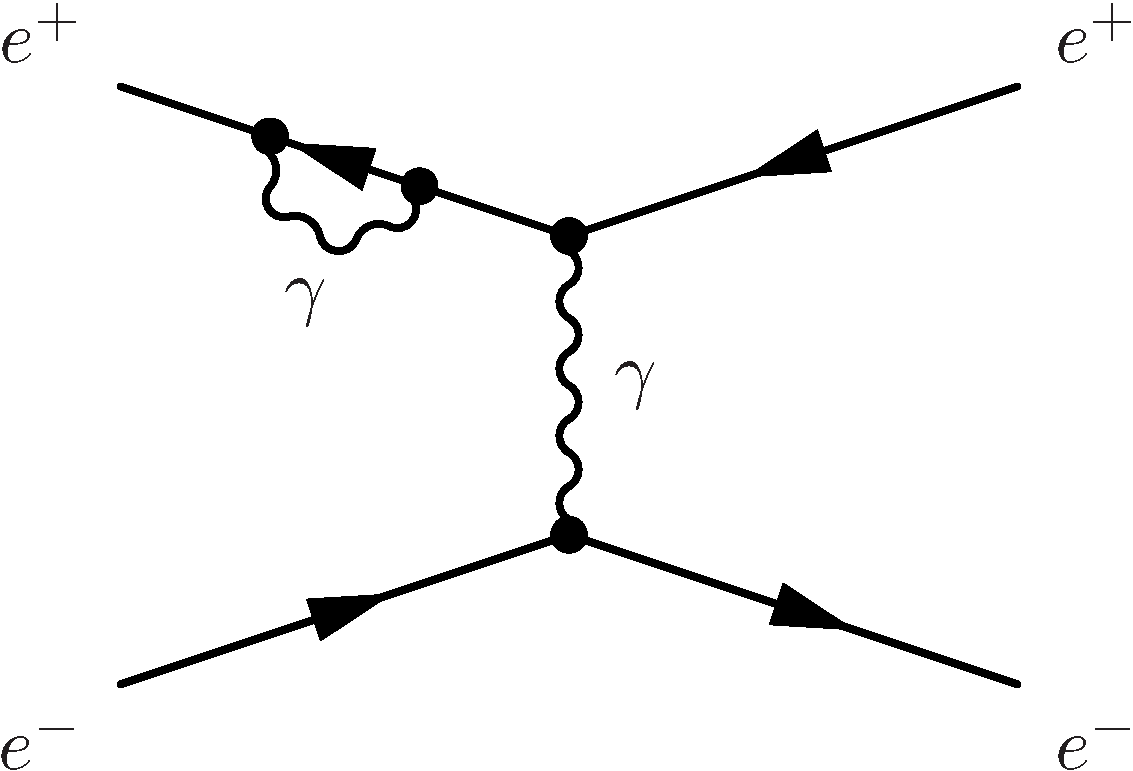
\includegraphics[width=.3\textwidth]{pics/self_energy}
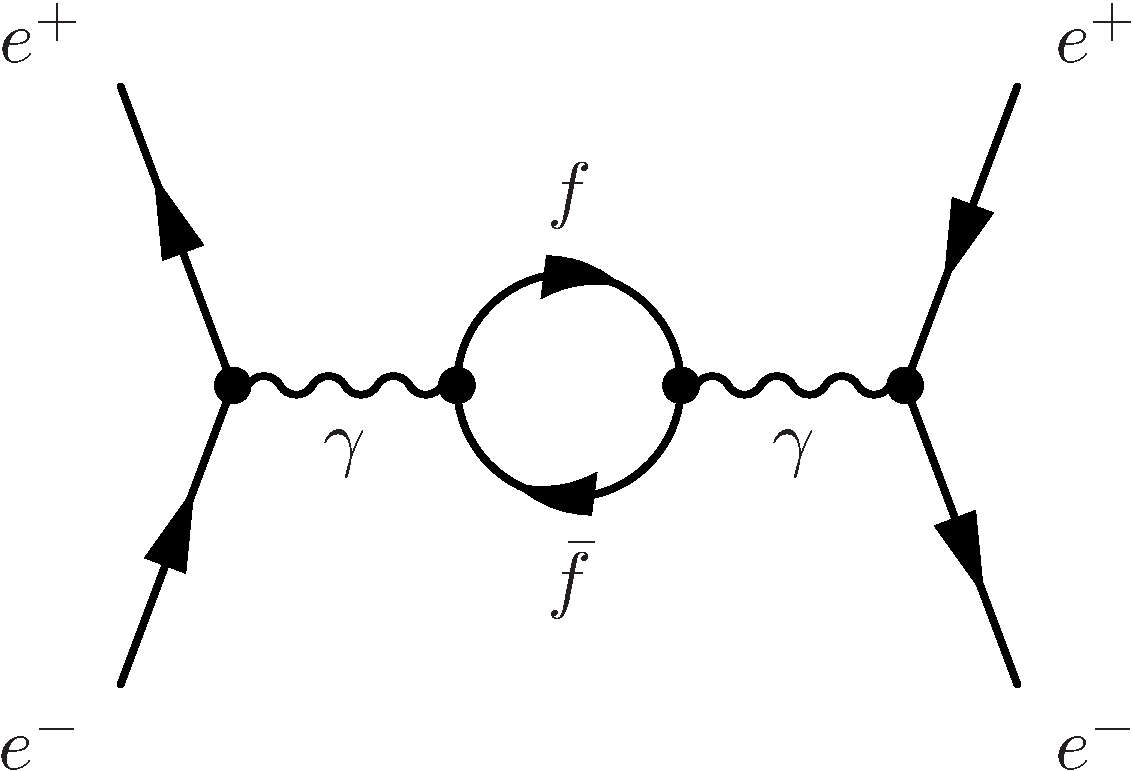
\includegraphics[width=.3\textwidth]{pics/mass_correction}
\end{center}
\caption{Radiative corrections at one loop in electron scattering. Time is directed horizontally. The vertex correction for interaction strength (left). The self-energy correction for the electron (middle)  
The photon self-energy propogator correction (right) }
\label{fig:one_loop}
\end{figure}

The perturbative expansion of the scattering matrix introduces momenta unconstrained by the in-going and out-going momentum and must be integrated out in our calculation of a scattering amplitude (Figure \ref{fig:one_loop}). In principle, these diagrams would be integrated up to infinity which leads to infinite matrix elements (which is clearly unphysical). The
means of how to deal with these infinite contributions to a matrix element is known as renormalization. The method of 
Renormalization was a historical triumph of quantum field theory as a tool of describing high energy particle physics.
 In the Wilsonian perspective of Renormalization, an effective theory like the Standard Model would only integrate
 over momentums below some finite energy scale where
 we expect the theory to no longer valid $\Lambda$ i.e. the cut off. This
 scale has important consequences for the theory. All dimensionful parameters of the theory will be expressed in terms of $\Lambda$ times constants which must be tuned against the cutoff. The level to which these constants must
 be tuned is known as the ``natural"-ness of the theory. 

\begin{figure}
\begin{center}
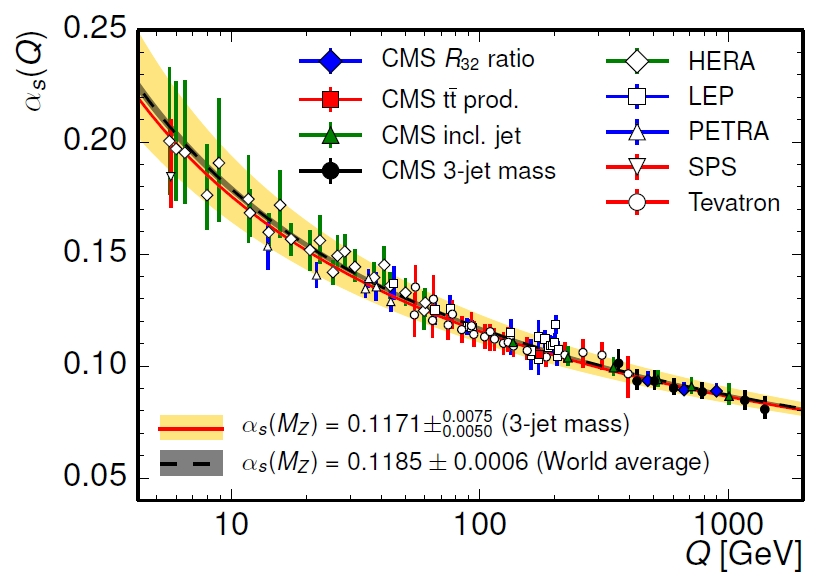
\includegraphics[width=.45\textwidth]{pics/alpha_s}
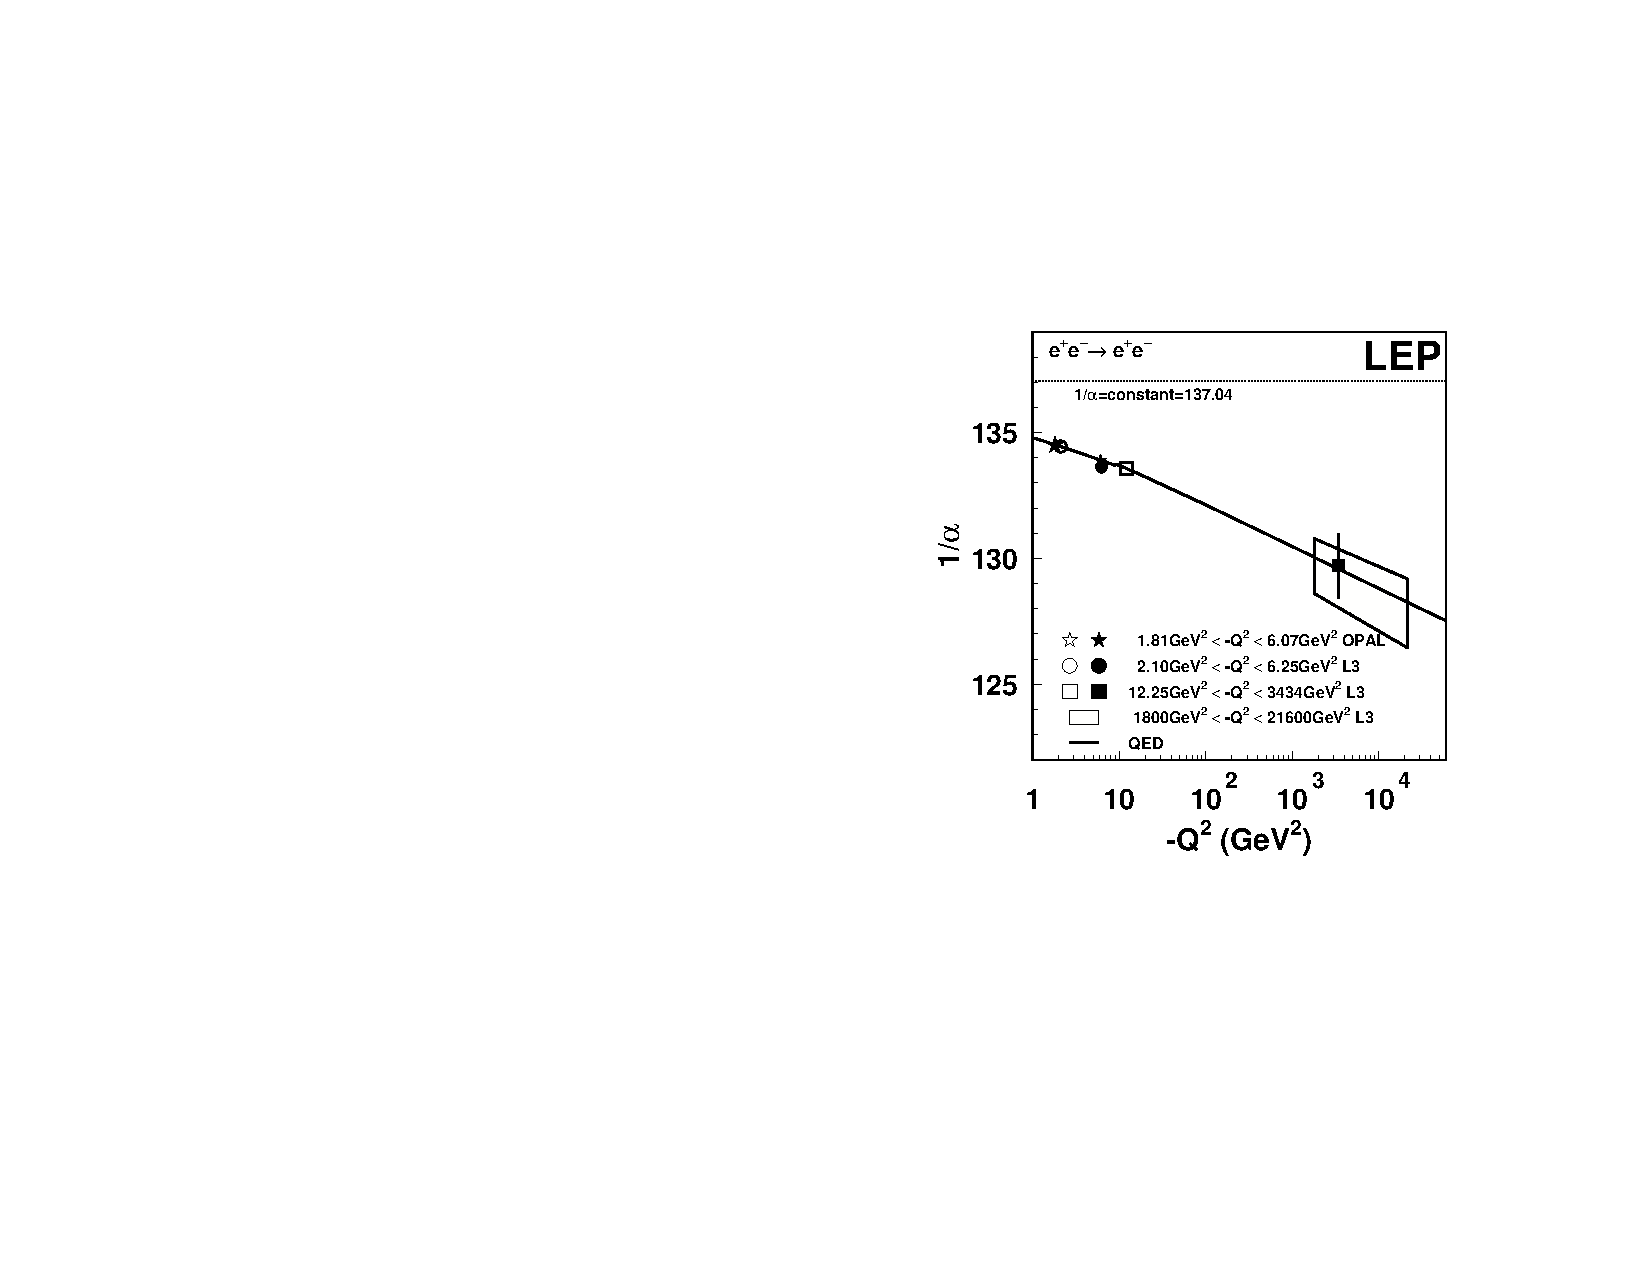
\includegraphics[width=.45\textwidth]{pics/alpha_qed}
\end{center}
\caption{}
\label{fig:running_coupling}
\end{figure}

Examples of 1 loop diagrams are shown in Figure \ref{fig:one_loop}. These diagrams have important consequences on the
experimentally measured values of the parameters of the theory. The first diagram gives a correction to the electroweak coupling strength and the electron magnetic moment. The second and thrid diagram induce corrections to the electron and photon propagator, respectively. An important consequence is the parameters of the theory, like the coupling, will effectively change ( ``run'') with the momentum $q^2$ with which the process is taking place. Historically, exepriments (Figure \ref{fig:running_coupling}) have confirmed the $q^2$ dependence of the couplings $\alpha_s, \alpha$. Additionally, these loops will have contributions from all possible verticies in the lagrangian, not just the flavors and families included in the in and 
out going states. intrestingly, the largest uncertainty in precision electroweak theory comes from hadronic loop contirbutions.

When  dimensional analysis is performed on lagrangian terms with mass dimension greater than 4, say $\frac{g}{5!}\phi^5$ 
we see that because the action is dimensionless and the coupling constant $g$ must have dimension $1/M$. As the only
mass scale in the theory is $\Lambda$ (of which all other mass scales can be written),  
the coupling will scale as $1/ (c \Lambda)$ where $c$ is some dimensionless number. 
When the scales probed by the theory are small compared to cuttoff $q^2/\Lambda^2 \rightarrow 0$
 these terms are irrelavent in the theory. If the higher dimensional operators existed, we would only
see evidence when probing energies $q^2 \sim \Lambda^2$.  This would be evidence of new physics to 
be incoperated and a subsequent increase of the value of $\Lambda$ to where the new theory would break down. 

\begin{figure}
\begin{center}
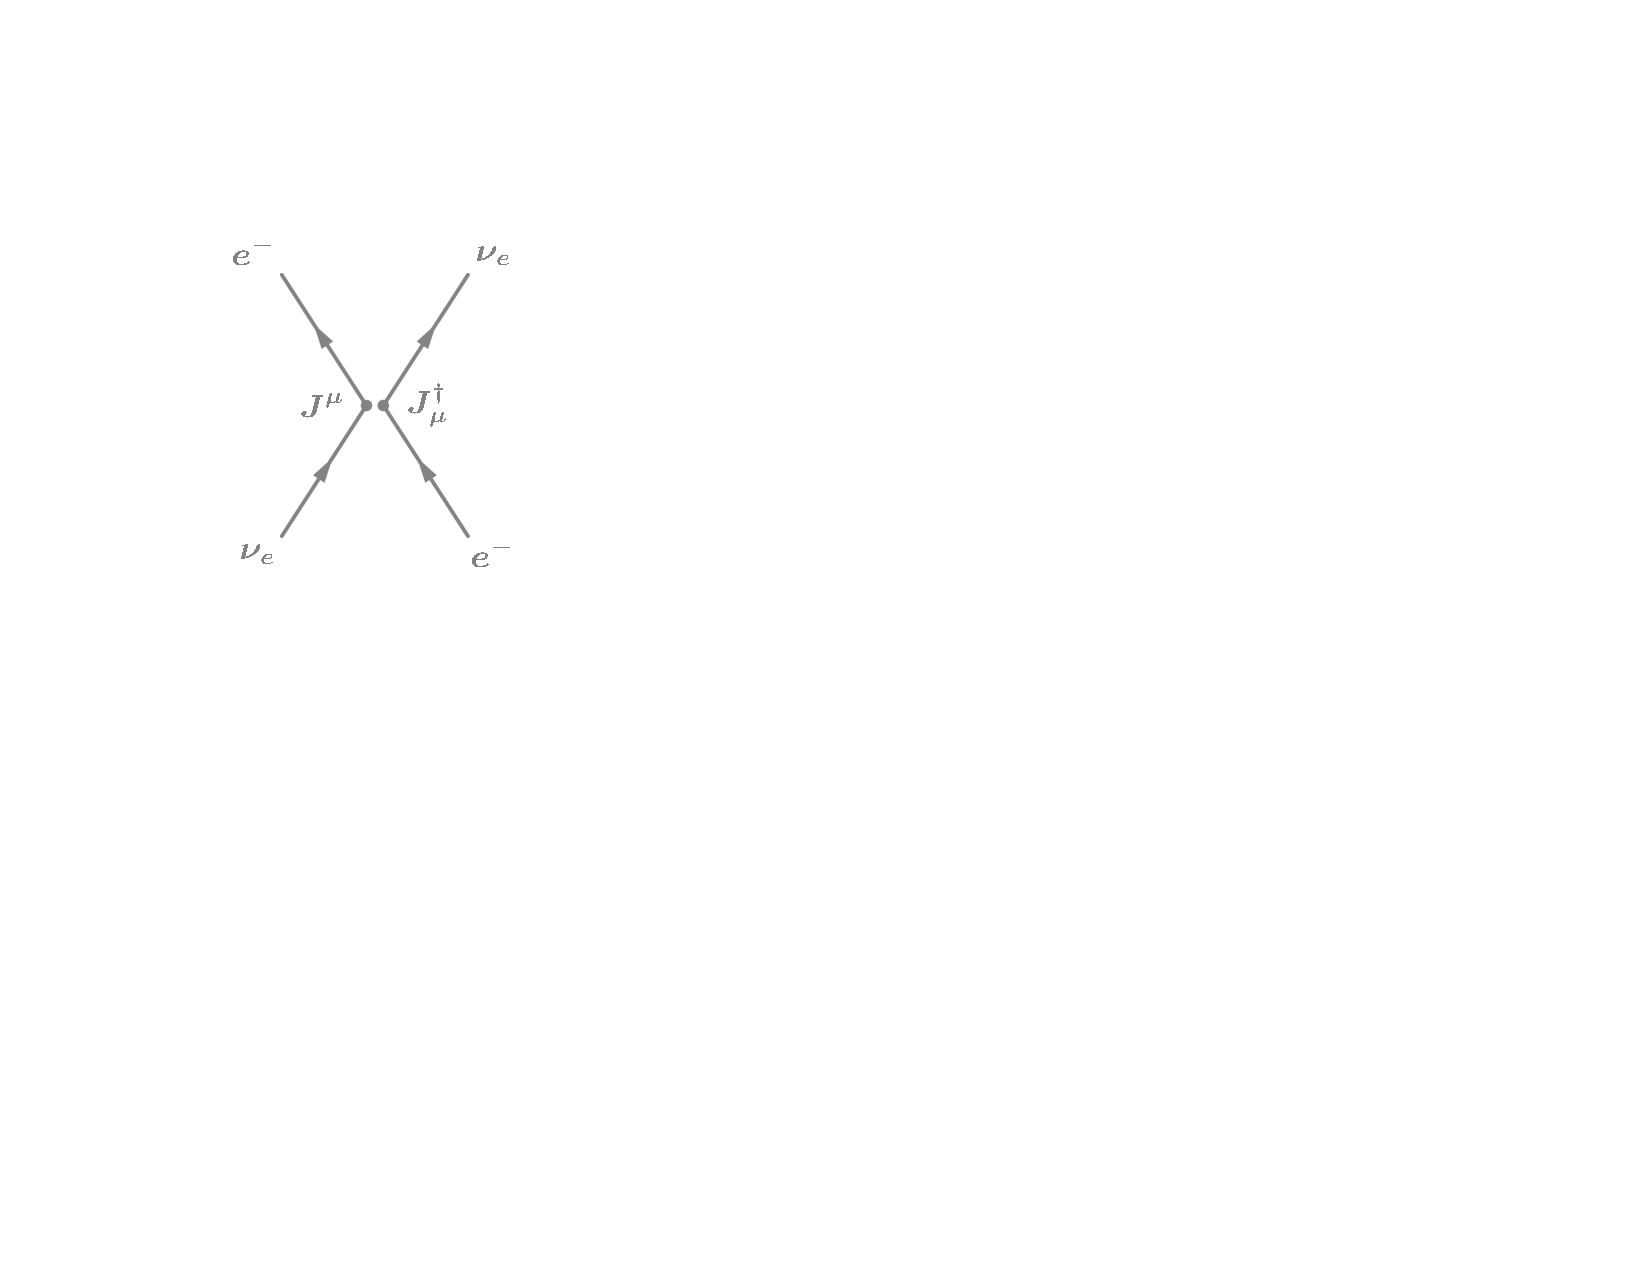
\includegraphics[width=.25\textwidth]{pics/fermi_theory}
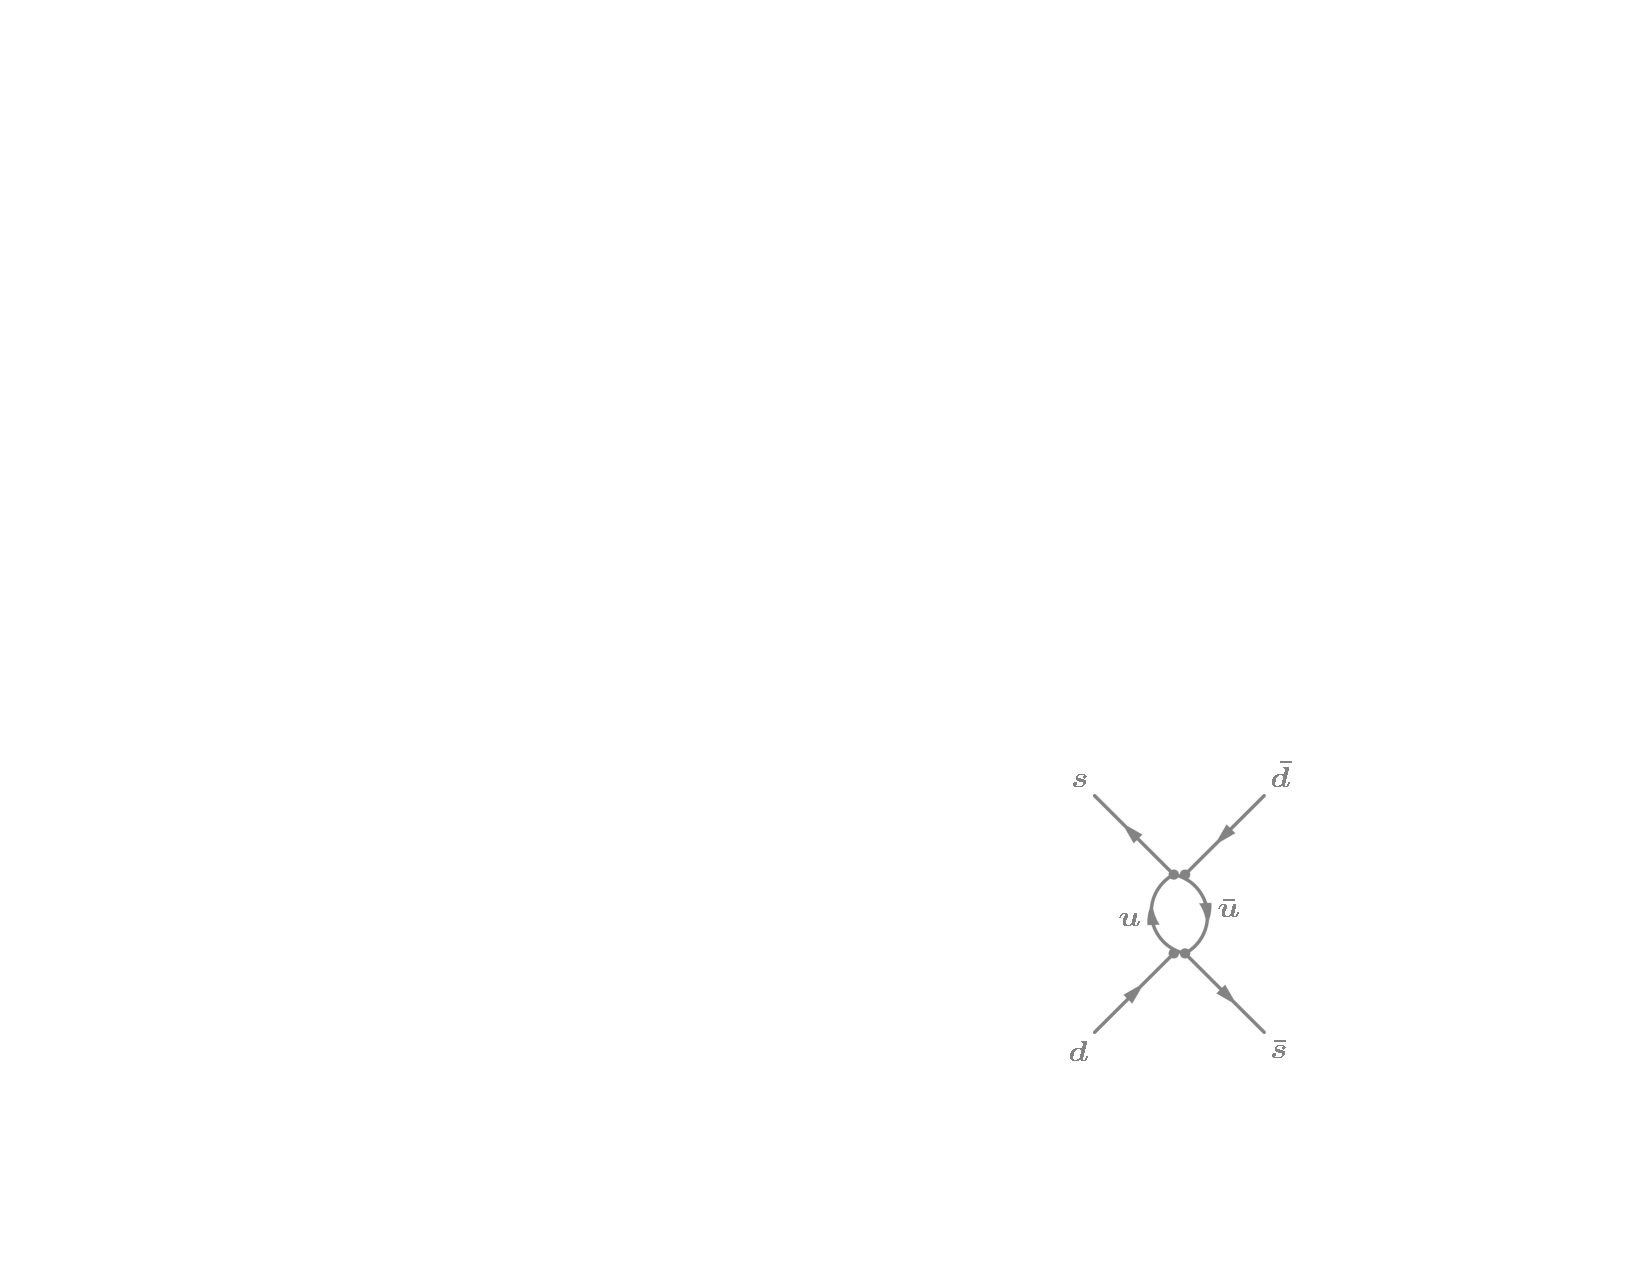
\includegraphics[width=.25\textwidth]{pics/fermi_diverge_ds}
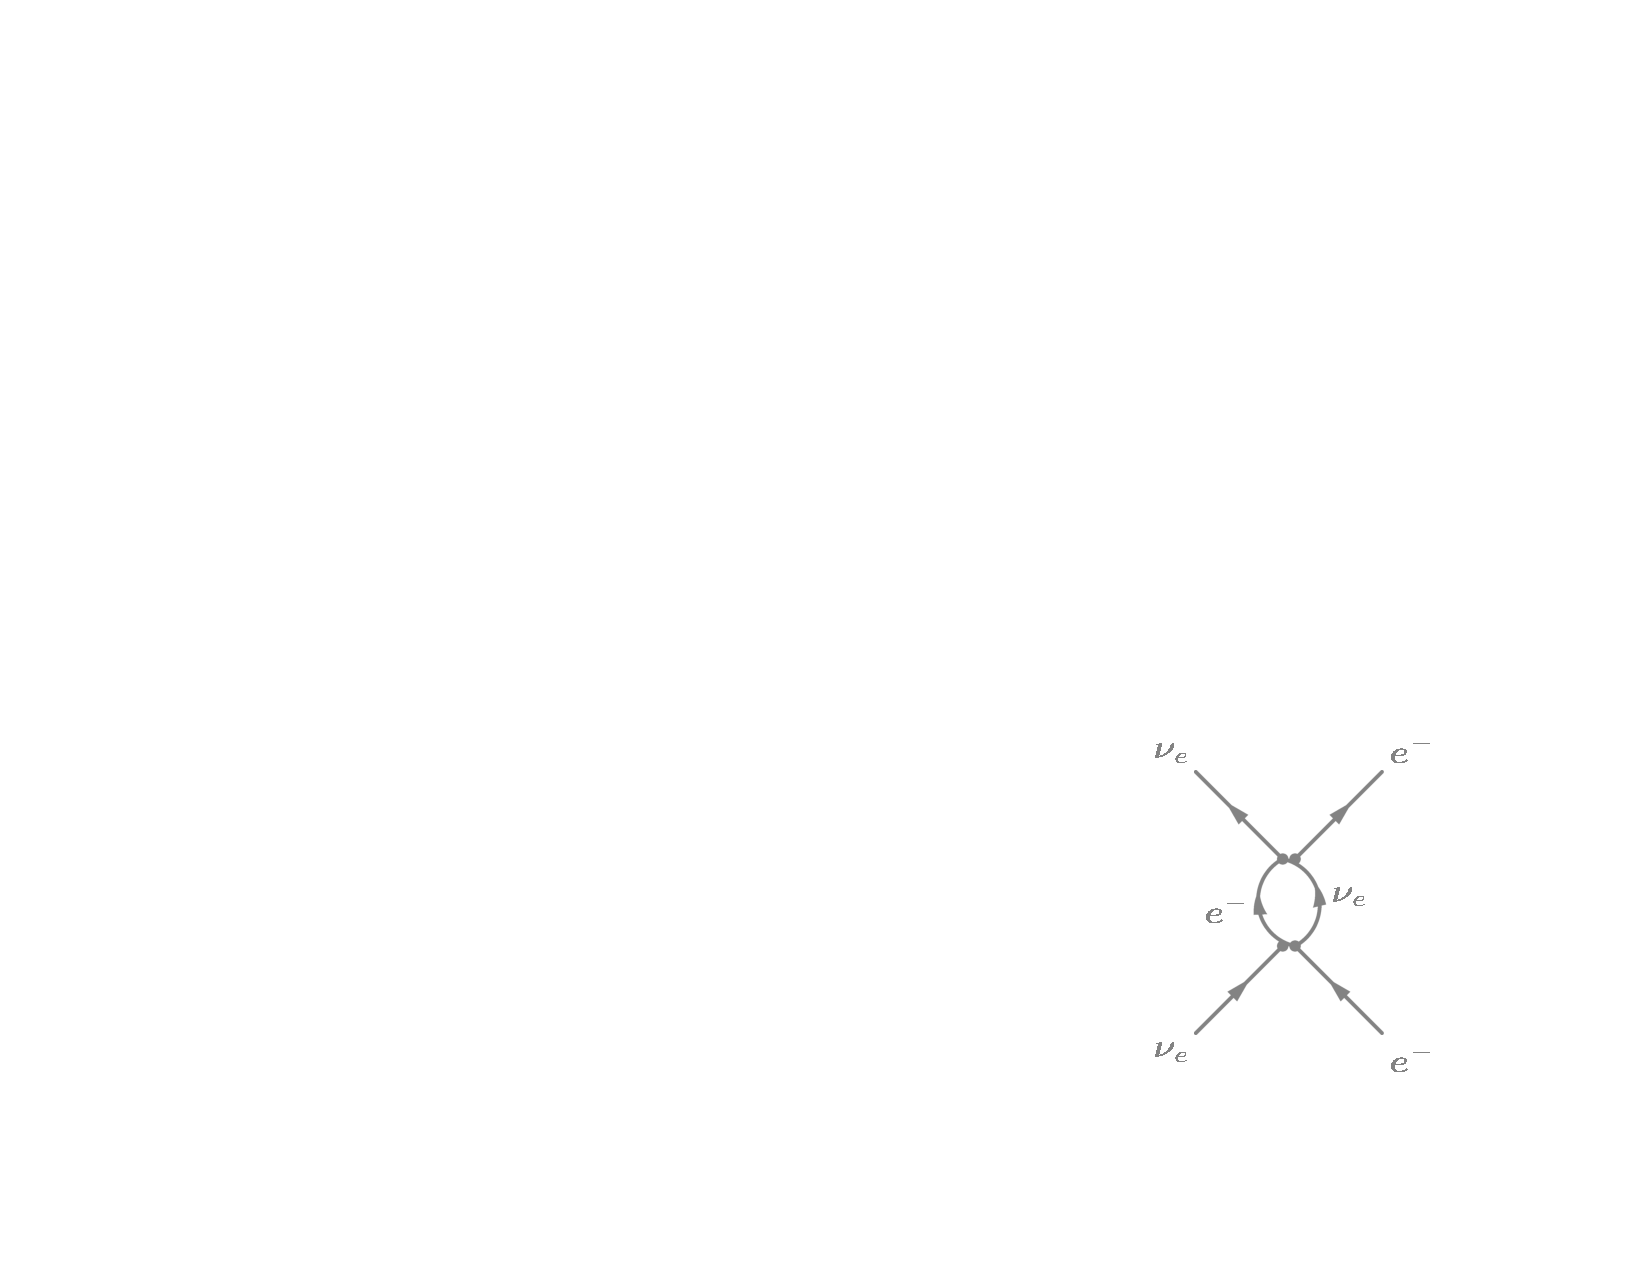
\includegraphics[width=.25\textwidth]{pics/fermi_divergence}
\end{center}
\caption{}
\label{fig:fermi_divergence}
\end{figure}

As a concrete example, we consider the four point Fermi interaction which models electroweak theory as a contraction
 of hadronic and leptonic currents 
\begin{align*}
-\mathcal{L}  &= \frac{G_F}{\sqrt{2}} J^\dagger_\mu J^\mu  \text{ with } J_\mu = J^l_\mu + J^{had}_\mu\\
J_\mu^l &= \bar{e}^- \gamma_\mu (1- \gamma^5) \nu_e + \bar{\mu} \gamma_\mu (1- \gamma^5) \nu_\mu \\
J_\mu^{had} &= \bar{u} \gamma_\mu (1- \gamma^5) d'
\end{align*}
These diagrams are capable of describing a variety of processes correctly at tree level(cite-langacker):
\begin{itemize}
\item Neutron $\beta$ decay $n\rightarrow p e^-\bar{\nu}_e$
\item $\mu,\tau$ decay $\mu^- \rightarrow e^- \bar{\nu}_e \nu_\mu$ $\tau\rightarrow \mu^- \bar{\nu}_\mu \nu_\tau$ 
\item $\pi,K$ decay $\pi^+ \rightarrow \mu^+ \nu_\mu$ 
\item heavy quark decays $c \rightarrow s e^+ \nu_e$ and  $b \rightarrow c \mu^- \bar{\nu}_\mu$ 
\end{itemize}
Despite these successes at tree level, the theory has divergent diagrams (Figure \ref{fig:fermi_divergence}) at one loop
\begin{align*}
\int d^4k \left ( \frac{k_\mu \gamma^\mu}{k^2} \right ) \left ( \frac{k_\mu \gamma^\mu}{k^2} \right ) \sim \int dk k  \sim \Lambda^2 
\end{align*}
Since a fermion has $[\psi] \sim [M]^{3/2}$ the coupling $G_F$ must have dimension $[M]^{-2}$ and therefore
non-renormalizable. New physics at the electroweak scale was needed. Today we know these diagrams needed an 
 intermediate vector boson (Figure \ref{fig:int_vec_boson}) to be UV complete. The $[M]^{-2}$ dependence
of the $G_F$ is precisely due to the $W$ propagating mass:
\begin{align*}
G_F \frac{\sqrt{2}}{8} \frac{g_W^2}{m_W^2} \text{ with } m_W\aprox 80 \text{ GeV and } g_W = 0.65
\end{align*}

\begin{figure}
\begin{center}
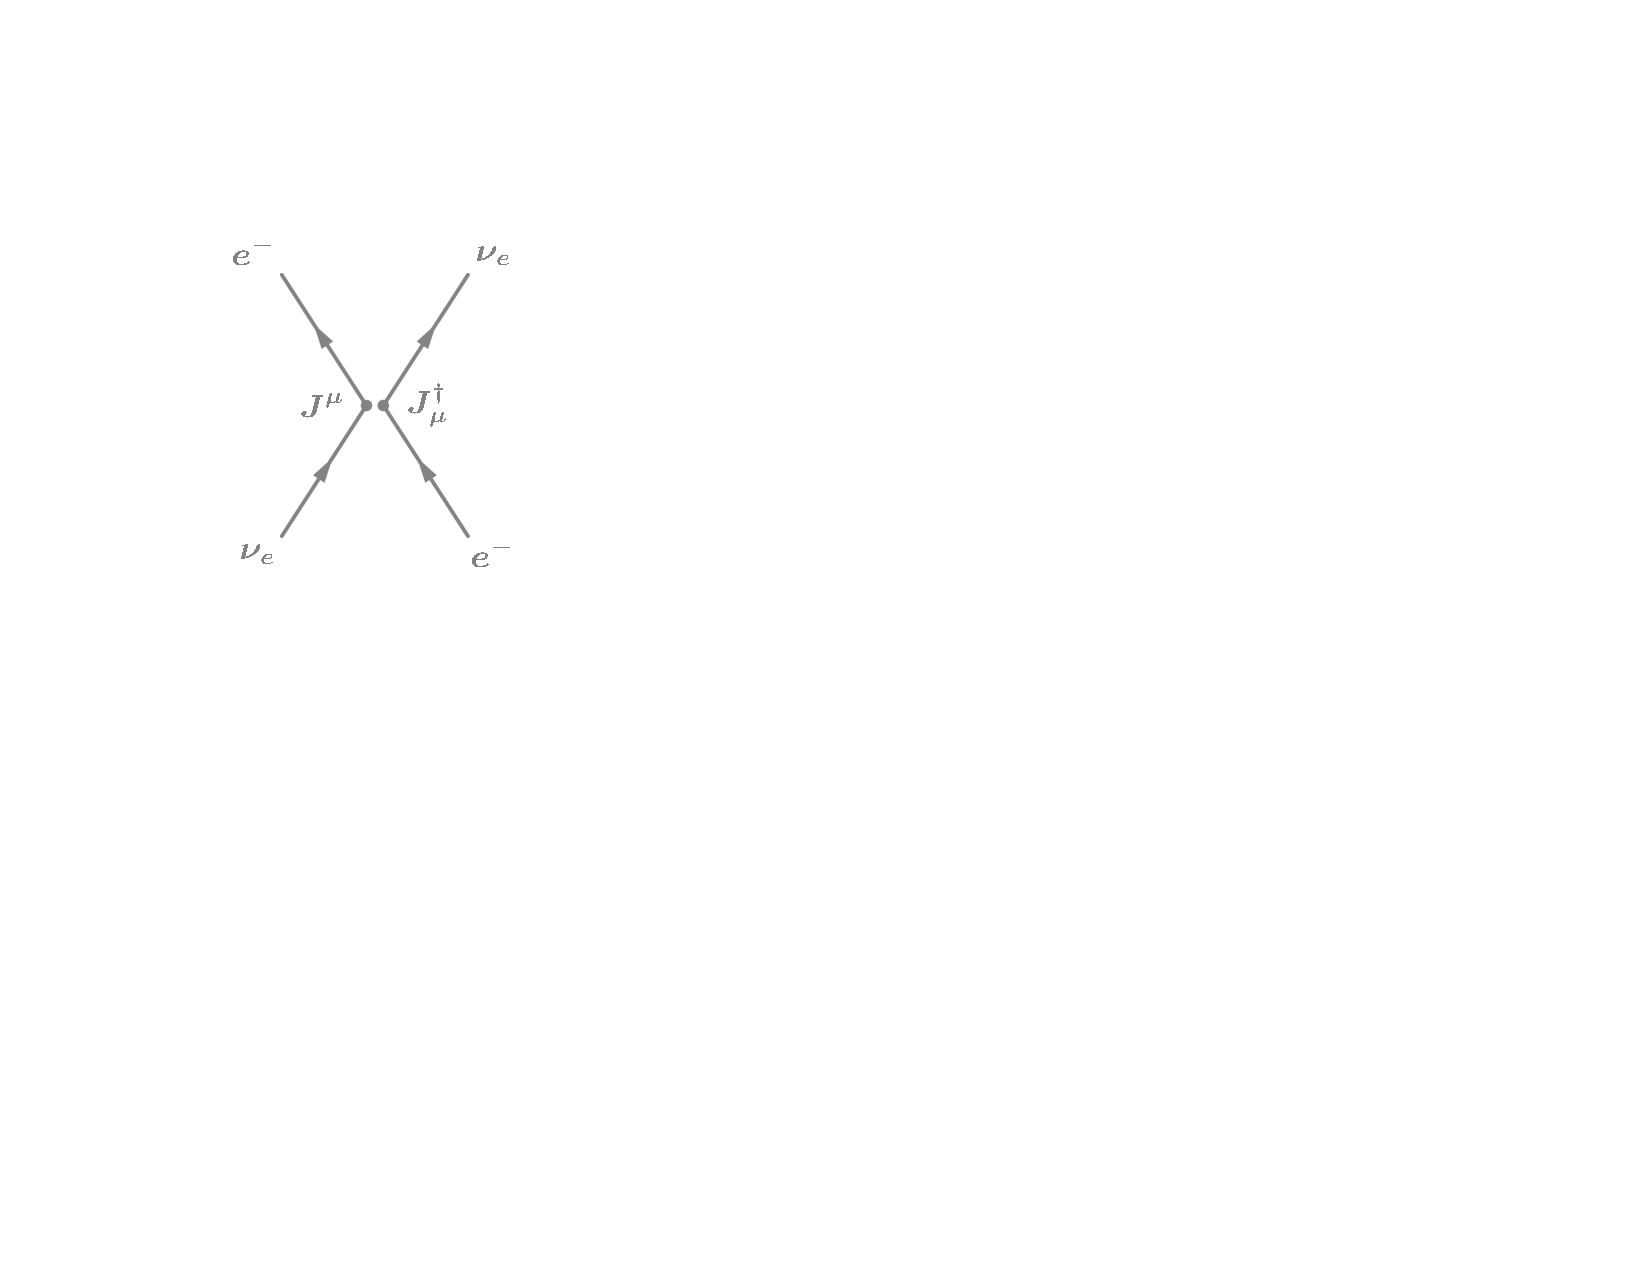
\includegraphics[width=.25\textwidth]{pics/fermi_theory}
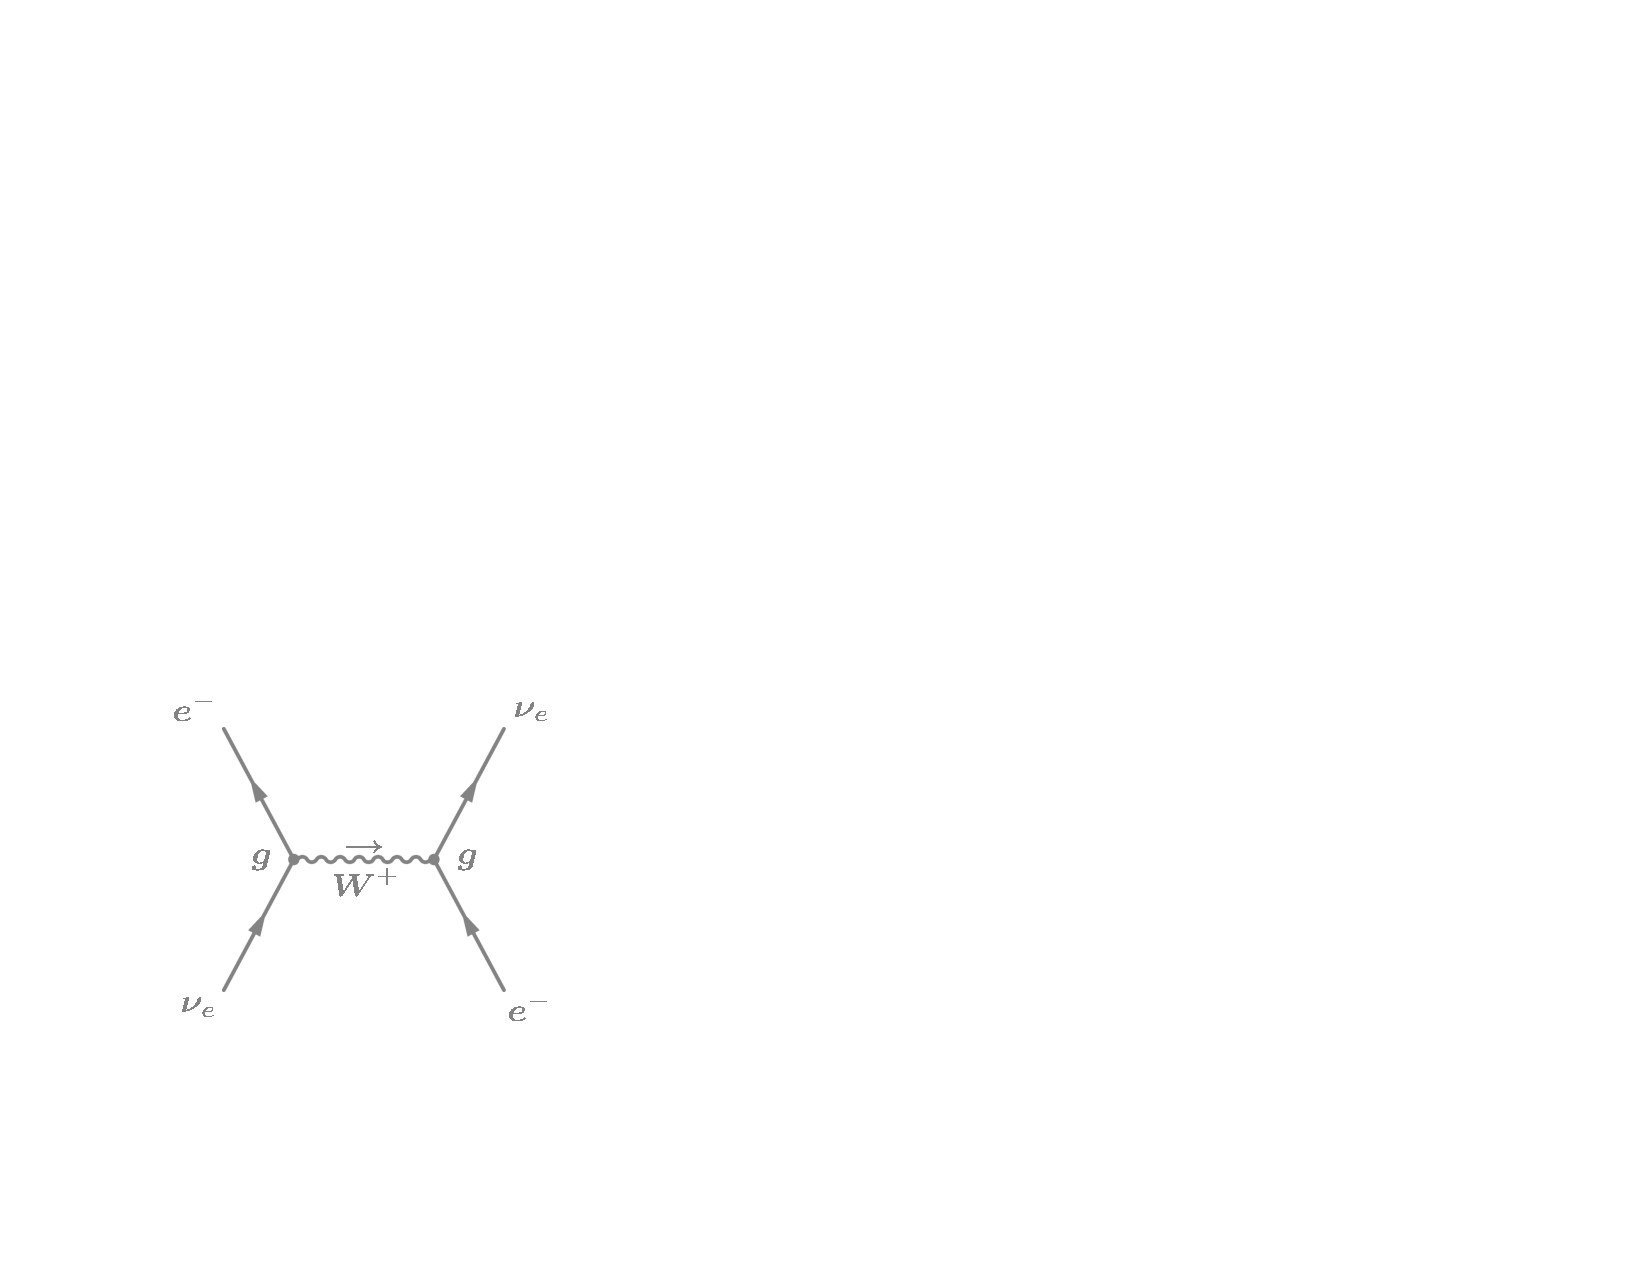
\includegraphics[width=.35\textwidth]{pics/int_vec_boson}
\end{center}
\caption{The four fermi theory for the weak interaction in terms of currents $J^\mu$ (left) is realized in the standard model through a three point function including intermediate vector boson propogator (right)}
\label{fig:int_vec_boson}
\end{figure}


\section{Supersymmetry}

The expectation of discovering supersymmetry (SUSY) at the TeV scale has been largely motivated
 by arguments based on naturalness. 
Since the mass of the Standard Model Higgs boson is sensitive to the high energy scale where SUSY
 is broken ($m_{SUSY}$), its mass, of order the electroweak scale, $(m_h \approx m_{EW} \ll m_{SUSY})$
 would need to be tuned to order $m_{EW}^2/m_{SUSY}^2$. 
To avoid fine-tuning, we would like  $m_h^2 \approx m_{SUSY}^2 \implies m_{SUSY} \leq$ 1 TeV. 
More specifically, knowing $m_H \approx 125$ GeV we expect light SUSY partners (in particular, light stops)
 near $< 1$ TeV to stabilize the quadratic divergences of 1 loop corrections to the Higgs mass
 [citation:$light_stops$]. 
Unfortunately these scalar partners have yet to be discovered.

It is important to note that the stability of the Higgs boson mass is not the only
 fine-tuning problem in particle physics. 
When the same argument is made for the cosmological constant we arrive at $\Lambda \geq m_{SUSY}^4$, 
where experimentally $\Lambda = 10^{-59}$ TeV$^4$.   
If we use the same SUSY scale as we did for the Higgs mass,
 $m_{SUSY} = 1$ TeV we have a new fine tuning problem of $10^{60}$.


\section{Long-lived Signatures}

\subsection{Standard Model Particles with Long Lifetimes}

The standard model already includes a variety of particles that can generate
 displaced vertices (Table \ref{tab:mesons} Table \ref{tab:baryons}). 
For example, $B^0 \rightarrow J/\psi K^{*0}$ with $K^{*0} \rightarrow K^+\pi^-$ 
generates a 4 track vertex. Such a vertex is commonly utilized 
in b-tagging. Of particular interest to single displaced jet identification outside of the b-tagging regime are charge neutral SM particles
decaying to charged particles with a few centimeter lifetime: $\Lambda^0$, $K_S^0$. Such particles would have no track
leading to the primary vertex and vertices far outside the b lifetime. The most relevant of processes being:

\begin{enumerate}
\item $K_s^0 \rightarrow \pi^+\pi^-$ 69\% of all $K_s^0$ decays 
\item $\Lambda^0 \rightarrow p \pi^-$ 64\% of all $\Lambda^0$ decays 
\end{enumerate}

Jets containing prompt and non-prompt $K_s$ and $\Lambda^0$ will contain tracks with large impact parameters, 
and large impact parameter significance. When a vertex is fit to the matched tracks we expect small track multiplicity relative 
to the GeV to TeV   long-lived particles this identification targets. It is important to separate this contribution from
the detector effects like nuclear interactions.

\begin{table}
\begin{center}
\begin{tabular}{cccccc}
\hline
\textbf{Name}  & \textbf{Content}                                    & \textbf{Particle}    & \textbf{mass} (MeV) & $\tau_{0}$ (sec)  & c$\tau$ (cm)         \\
\hline 
Pion & $u\bar{d}$                                  & $\pi^{\pm}$ & 139        & $2.6 \times 10^{-8}$       & $7.8 \times 10^{2}$  \\
\hline 
Kaon  & $u\bar{s}$                                 & $K^{\pm}$   & 497        & $     1.23 \times 10^{-8}$ & $3.7 \times 10^2$    \\
K Short  & $\frac{1}{\sqrt{2}}(d\bar{s} - s \bar{d})$ & $K^0_{s}$   & 497        & $0.896 \times 10^{-10}$    & 2.68                 \\
K Long  & $\frac{1}{\sqrt{2}}(d\bar{s} + s \bar{d})$ & $K^0_L$     & 497        & $5.1\times 10^{-8}$        & $1.5 \times 10^3$    \\
\hline
D & $c\bar{d}$                                 & $D^{\pm}$   & 1869       & $1 \times 10^{-12}$        & $3.0 \times 10^{-2}$ \\
\hline
B meson  & $u \bar{b}$                                & $B^{\pm}$   & 5279       & $1.6 \times 10^{-12}$      & $4.8 \times 10^{-2}$ \\
strange B  & $s\bar{b}$                                 & $B^{0}_s$   & 5366       & $1.5 \times 10^{-12}$      & $4.5 \times 10^{-2}$ \\
charmed B  & $c\bar{b}$                                 & $B^{0}_c$   & 6275       & $4.5\times 10^{-13}$       & $1.4 \times 10^{-2}$ \\
\end{tabular}
\end{center}
\caption{Mesons with Lifetimes greater than $10^{-2}$ cm} 
\label{tab:mesons}
\end{table}


\begin{table}
\begin{center}
\begin{tabular}{cccccc}
\textbf{Name}          & \textbf{Content} & \textbf{Particle}      & \textbf{mass} [MeV] &  $\tau_{0}$ [s] & $c\tau_{0}$ [cm] \\
\hline 
Lambda        & $uds$   & $\Lambda^0$   & 1115       & $2.6 \times 10^{-10}$    & 7.8                  \\
bottom Lambda & $udb$   & $\Lambda^0_b$ & 5620       & $1.4 \times 10^{-12}$    & $4.2 \times 10^{-2}$ \\
\hline
Sigma plus    & $uus$   & $\Sigma^{+}$  & 1189       & $8 \times 10^{-11}$      & 2.4                  \\
Sigma minus   & $dds$   & $\Sigma^{-}$  & 1197       & $1.4\times 10^{-10}$     & 4.2                  \\
\hline 
Xi zero       & $uss$   & $\Xi^0$       & 1314       & $4 \times 10^{-13}$      & $1.2 \times 10^{-2}$ \\
Xi minus      & $dss$   & $\Xi^-$       & 1321       & $1.6 \times 10^{-10}$    & 4.8                  \\
charmed Xi +  & $usc$   & $\Xi^{+}_c$   & 2467       & $4.42 \times 10^{-13}$   & $1.3 \times 10^{-2}$ \\
charmed Xi    & $dsc$   & $\Xi^0_c$     & 2471       & $1.12 \times 10^{-13}$   & $3.3 \times 10^{-2}$ \\
bottom Xi     & $dsb$   & $\Xi^-_b$     & 5792       & $1.56 \times 10^{-12}$   & $4.7 \times 10^{-2}$ \\
\hline
bottom Omega  & $ssb$   & $\Omega_b^-$  & 6054       & $1.13 \times 10^{-12}$   & $3.3 \times 10^{-2}$ \\
Omega minus   & $sss$   & $\Omega^-$    & 1672       & $8 \times 10^{-11}$      & 2.4                  \\
\end{tabular}
\end{center}
\caption{Baryons with Lifetimes greater than $10^{-2}$ cm} 
\label{tab:baryons}
\end{table}


Particles of a characteristic lifetime $\tau$ decay with a falling exponential. For reference, 
a table describing the percent of decays that will occur at various distances is shown in Table
 \ref{tab:lifetime}. Even lifetimes 10 and 100 times the size of the tracker, we would still expect
~10\% and 1\% respectively to occur within the tracker. For particles  of lifetime $\lambda$ we
expect 0.6\% to decay beyond $5\lambda$. 


\begin{table}
\begin{center}
\begin{tabular}{ccc}
Distance ($\lambda$) &  Probability of Decay  \\
\hline
0.01               & 1\%                        \\
0.1                & 9.5\%                      \\              
0.25               & 22\%                       \\            
0.5                & 39\%                       \\          
0.75               & 52\%                       \\        
1                  & 63\%                       \\      
1.5                & 77\%                       \\    
2                  & 86\%                       \\  
3                  & 95\%                       \\
5                  & 99.3\%                     \\
\end{tabular}
\end{center}
\caption{ A reference table for the cumulative probability for a particle of lifetime $\lambda$ to have decayed after a given
distance. Distance is in multiples of lambda.}
\label{tab:lifetime}
\end{table}


\subsection{Split-Susy and Naturalness at the LHC}

As addressed by Arkani-Hamed and Dimopoulos [citation:$nima_lhc$], many theoretical approaches  have been
 motivated by a natural explanation for the Higgs mass while separately seeking an  explanation
 of the cosmological constant through some other mechanism.
Arkani-Hamed and Dimopoulos propose a reconsideration of naturalness, entertaining the idea that 
fine tuning could have a role to play in beyond the Standard Model physics.
Conceivably, both $\Lambda$ and $m_h$ fine tuning could be resolved by the same mechanism.  
This un-natural model was  further investigated by Giudice and Romanino [citation:$split_susy$]
and dubbed ``split supersymmetry". 

Split SUSY assumes a much higher SUSY scale $m_{SUSY}^2 \gg 1$ TeV where all scalars (excluding the Higgs) 
become very heavy $O(m_{SUSY})$ and the lightest sparticles (Higgsinos and gluinos) are kept at the TeV scale by requiring the lightest neutralino to be a good dark matter candidate. 

Because the scalars are so much heavier, the decay of gluinos through squarks is suppressed.
The characteristic signature of split supersymmetry is thus long-lived gluinos; such processes 
with long lifetimes are rare in the SM.
